%\documentclass[sigconf,anonymous]{acmart}
\documentclass[a4paper,english]{lipics-v2018}
%\usepackage{microtype}%if unwanted, comment out or use option "draft"
%\settopmatter{printfolios=true,printccs=false,printacmref=false}
%\usepackage{balance}  % for  \balance command ON LAST PAGE  (only there!)
\usepackage{color}
\usepackage{subcaption}
\usepackage{algorithm}
\usepackage[noend]{algpseudocode}
\usepackage{graphicx}
\usepackage{amssymb}
\usepackage{url}
\usepackage{multicol}
\usepackage{booktabs} % For formal tables
\usepackage{times}

%\setcopyright{none}
%\acmConference{Submitted to SIGIR}{2018}{} 
%\acmYear{2018}

\usepackage{multicol}
\newcommand{\commentOut}[1]{}
\newcommand{\MaxScore}{maxScore}
\newcommand{\firstPosting}{firstPosting}
\newcommand{\pBMW}{pBMW}
\newcommand{\pRA}{pRA}
\newcommand{\pNRA}{pNRA}
\newcommand{\sNRA}{sNRA}
\newcommand{\pJASS}{pJASS}


\newcommand{\DHeap}{\textit{docHeap}}
\newcommand{\DMap}{\textit{docMap}}
\newcommand{\LDMap}{\textit{tmpDocMap}}
\newcommand{\TMap}{\textit{termMap}}
\newcommand{\Docobj}{\textit{DocType}}
\newcommand{\nil}{\bot}
\newcommand{\Done}{\textit{done}}
\newcommand{\RAStop}{\textit{UBStop}}
\newcommand{\HeapUpdateTime}{\textit{heapUpdTime}}

\newcommand{\ex}{-exact}
\newcommand{\hi}{-high}
\newcommand{\lo}{-low}

\newcommand{\cw}{ClueWeb}
\newcommand{\cwten}{ClueWebX10} 

\newcommand{\alg}{Sparta}  
\newcommand{\inred}[1]{{\color{red}{#1}}}
\newcommand{\inblue}[1]{{\color{blue}{#1}}}
\newcommand{\remove}[1]{}

\bibliographystyle{plainurl}% the recommnded bibstyle

\nolinenumbers

% ****************** TITLE ****************************************

\title{Fast Parallel Top-K Retrieval of Verbose Queries}

%\titlerunning{Dummy short title}%optional, please use if title is longer than one line

\author{Gali Sheffi}{Yahoo Research, Oath}{gsheffi@oath.com}{}{}
\author{Dmitry Basin}{Yahoo Research, Oath}{dbasin@oath.com}{}{}
\author{Edward Bortnikov}{Yahoo Research, Oath}{ebortnik@oath.com}{}{}
\author{David Carmel}{Amazon}{david.carmel@gmail.com}{}{}
\author{Idit Keidar}{Technion and Yahoo Research, Oath}{idish@ee.technion.ac.il}{}{}

\authorrunning{Sheffi et al.}

\Copyright{Gali Sheffi and Dmitry Basin and Edward Bortnikov and David Carmel and Idit Keidar}%mandatory, please use full first names. LIPIcs license is "CC-BY";  http://creativecommons.org/licenses/by/3.0/

\subjclass{C.1.4 Parallel Architectures and D.1.3 Concurrent Programming}% mandatory: Please choose ACM 2012 classifications from https://www.acm.org/publications/class-2012 or https://dl.acm.org/ccs/ccs_flat.cfm . E.g., cite as "General and reference $\rightarrow$ General literature" or \ccsdesc[100]{General and reference~General literature}. 

\keywords{Parallel computing, web-search, top-k}%mandatory

\begin{document}

\maketitle

\begin{abstract}
Top-k document retrieval is emerging as a performance bottleneck in query processing as verbose queries are becoming 
mainstream, while state-of-the-art algorithms fail to process such long queries in real time. To date, attempts to
accelerate top-k evaluation 
via approximate result computation and intra-query parallelism have produced limited results. 

We present \alg\ -- a practical parallel algorithm that exploits multi-core hardware to run approximate top-k retrieval 
within interactive latency bounds. Its design is inspired by  Fagin et al.'s seminal Threshold Algorithm for  aggregation in databases. 
\alg\ scales through lightweight coordination and context sharing among concurrent threads. The resulting algorithm 
is highly scalable, 
both in the number of query terms and in the searched index size. For example, when applied to the 50M-document public ClueWeb09B 
dataset, \alg\  processes $12$-term queries $3.6$ times faster than the state-of-the-art. On a tenfold  bigger index, 
\alg\ continues to process queries at the same speed, whereas today's best-in-class algorithm is more than 60 times slower. 
\alg\ further significantly improves throughput.% on production-motivated query mixes. 
\end{abstract}

\maketitle


\section{Introduction}
\label{sec:intro}

% Problem: long queries
% The reliance of Internet users on search engines became enormous during the past two decades. 
Internet users are changing the ways in which they interact with search engines. 
While  early days web queries were short (2.4 terms on average~\cite{Spink:2001:SWP:362968.362979}), 
modern search experiences (query suggestion, reformulation, conversational interfaces, etc.) stimulate their users to submit much longer queries. 
For example, more than 5\% of queries submitted via voice search on mobile devices exceed 10 terms~\cite{sigir/Guy16}. 
At the same time, usability studies
(e.g.,~\cite{Arapakis:2014:IRL:2600428.2609627}) show that users are extremely sensitive to end-to-end delays beyond 500 ms, 
and any excess delay beyond 250 ms leads to material degradation in their experience. Maintaining this \emph{service-level agreement} ({\em SLA}) 
is becoming a major challenge as more queries become longer.

 Most search systems today evaluate queries via a two-stage process~\cite{Wang:2011}. 
The first stage is \emph{top-k retrieval}: it 
 roughly matches the top-k documents most relevant to the query (typically, hundreds to thousands) based on some simple relevance scoring function like tf-idf or BM25~\cite{Baeza-Yates:1999:MIR:553876}. The second stage then re-ranks the  documents via some sophisticated (e.g., machine-learned) function, to produce the final result list (typically, a few tens of documents). 
The first stage  sifts through huge volumes of data and dominates the execution time. 
We therefore focus on the latency induced by this stage. 

%\inred{
The retrieval stage is typically executed in a backend  tier on dedicated search nodes, each of which retrieves the top-k results from a local index shard. 
With the advance of storage and memory technologies, the size of index shards increases, thus increasing the load on each search node. 
A promising approach to handle this load is to  parallelize query evaluation on multiprocessor hardware. 
The current trend in server architecture, which favors parallelism over sequential speed, makes this approach particularly attractive. 
We explore this approach in this paper.
%}


% Approximate is the only option
Obtaining the exact top-k matches out of a large corpus is typically too slow to meet stringent SLA requirements. 
Given that the top-k selection is only the first query  processing step, perfect results are often not essential, as later query processing 
stages can be satisfied by approximate results~\cite{Crane:2017,Lin:2015,Wang:2011}. 
Based on this observation we focus on \emph{approximate} 
(sometimes called \emph{non-safe}) query evaluation, tuned to achieve a certain high recall (e.g., $97\%$ or more). 
%of the original results).
% that is deemed sufficient for the application at hand. 

%Top-k retrieval algorithms have been  studied in the query processing literature~\cite{Baeza-Yates:1999:MIR:553876,
%Broder:2003:EQE:956863.956944, Ding:2011:FTD:2009916.2010048}. They capitalize on aggressive pruning of the search space, 
%in order to reduce the traversal time. 
State-of-the-art sequential algorithms for approximate top-k  retrieval, 
%which have both exact (safe) and approximate versions, 
e.g., \emph{Block-Max WAND} ({\em BMW})~\cite{Ding:2011}, serve traditional (short) web queries with impressive speed. 
However, these algorithms do not scale well to verbose queries
\bigdataset{
and big data collections 
}
(as pointed out in~\cite{Bortnikov:2017} and confirmed by our experiments). 
%
Parallelizing these algorithms can improve performance by 30\%--40\%~\cite{rojas2013efficient},    but 
%Rojas et al.~\cite{rojas2013efficient} propose a \emph{parallel} variant of BMW, which we call \emph{pBMW}, achieving 
%performance improvements of 30\%--40\%. 
% ;  we refer to their  algorithm as \emph{pBMW}. %-- with a considerable performance improvement.
our experiments show that such a parallel BMW implementation still has limited scalability, falling short of expected SLAs on long queries. 
%(e.g., 1 second for 
%12-term query over ClueWeb with eight threads, in our experiments). 
%The algorithm does not achieve high recall when stopped early. 

We present \emph{\alg} (Scalable PARallel Threshold Algorithm) -- a novel 
concurrent algorithm that substantially improves search time for verbose queries over large search indices. Its
%the tail
 query latencies fit well within  real-time SLAs on standard  server hardware. 

\alg's design is inspired by the seminal \emph{Threshold Algorithm (TA)} by Fagin et al.~\cite{Fagin:2003} for retrieving the top-k objects from a database based on an aggregation of attributes that may reside in multiple nodes. 
%%%%Perhaps surprisingly, this algorithm was largely ignored in the web search literature.
%, despite its relevance. 
In the web setting, term posting lists represent attributes and the ranking function is a linear aggregation of term scores. TA has two variants~\cite{Fagin:2003}: (1) \emph{Random Access} ({\em RA}), which  
 relies on random access to  posting lists; 
%\inred{Gali: shouldn't we mention that TA's "regular" posting lists are sorted by term scores?} 
and (2) \emph{No Random Access} ({\em NRA}), which 
 only traverses them sequentially. The former is ineffective in the context of real-time search 
because it requires (1)  a secondary random-access index (which doubles the required index space), 
and (2) random I/O to the on-disk secondary index, which incurs high overhead when the index  is too big to be 
kept entirely in RAM. We therefore base our algorithm on  NRA. 



Transforming NRA into an efficient concurrent algorithm is challenging because coordination around 
shared state can become a major bottleneck unless carefully designed. On the one hand,
sharing state among threads is essential in order to benefit from TA's early stopping feature.
Indeed, our experiments show  that a shared-nothing (partitioned) parallelization of NRA performs two times 
worse than a single-threaded implementation. On the other hand, 
a na\"ive attempt to parallelize NRA using shared memory also results in 
worse performance than the sequential algorithm. \alg\ judiciously shares 
information among threads while significantly reducing the synchronization 
overhead and memory overlap among them, 
%which results in efficient use of hardware resources, 
leading to major performance gains. 

Our results show that \alg\ scales well with 
\bigdataset{
both  corpus size and
}
query length.
E.g., on the 50M-document TREC ClueWeb09B dataset~\cite{ClueWeb09}, %\footnote{\url{https://lemurproject.org/clueweb09}}, 
\alg\ can serve verbose 12-term queries within less than 200 ms, 
whereas a parallel execution of RA processes them in 400 ms, and a parallel execution of BMW takes more than 600 ms. 
%Moreover, \alg\ scales much better with the corpus size:  
\bigdataset{
On a 500M-document index,  its latency is virtually unchanged, whereas 
 \pRA\ requires 2 seconds and pBMW's latency surges to almost 10 seconds.  
  The latter occurs because unlike \alg\ and \pRA, 
pBMW's processing time grows linearly with the index size.
}
%While \alg's advantages are most pronounced for long queries, its 
\alg's throughput on a production-grade query mix (with the query length distribution measured in~\cite{sigir/Guy16}) is twice that of parallel BMW.
\bigdataset{
 on the small corpus, and 25x faster on the large one.
}

Summing up, we present a practical scalable parallel algorithm that significantly improves the state-of-the-art latency  of long query processing.
\bigdataset{
on large search indices.
}
%
The paper proceeds as follows: Section~\ref{sec:problem} defines the top-k retrieval problem and associated metrics. 
Section~\ref{sec:background} gives background on existing algorithms. 
Section~\ref{sec:alg} presents \alg, and Section~\ref{sec:eval}  evaluates it.
Finally, 
Section~\ref{sec:related} discusses related work and Section~\ref{sec:conclusions} concludes the paper.

%%%%%%%%%%%%%%%%%%%%%%%%%%%%%%%%%%%%%%%%%%%%%%%%%%%%%%%%%%%%%%%%%%%%%%%%%%%%%%%%%%%%%
% Problem 
%%%%%%%%%%%%%%%%%%%%%%%%%%%%%%%%%%%%%%%%%%%%%%%%%%%%%%%%%%%%%%%%%%%%%%%%%%%%%%%%%%%%%

\section{Problem Statement: Top-k Retrieval}
\label{sec:problem}

We focus on the fundamental primitive of top-k retrieval, widely used in 
information retrieval, web search, data mining, data analytics, and more~\cite{top-k-survey}. 
This primitive is commonly used for initial selection of documents over which more refined search is performed~\cite{Wang:2011}. 
%The primitive uses a scoring function, denoted as $\textit{score}(D, q)$, that scores each document
%$D$ based on an estimation of its relevance to the query $q$.

Given a query $q$, the primitive retrieves the top $k$ scored  \emph{documents} (data items) in a given corpus
according to a scoring function $\textit{score}(D, q)$.  
%More specifically, 
A \emph{query} is given as a list of terms (features). Given an $m$-term query $q = t_1, \dots t_m$ and a document $D$, the score of $D$ for query $q$ is 
%\begin{equation} \label{eq:score}
$\textit{score}(D, q) \triangleq \sum_{i=1}^m ts(D, t_i)$ 
%\nonumber
%\end{equation}
%\[ \textit{score}(D, q) \triangleq \sum_{i=1}^m ts(D, t_i).\]  
where $ts(D, t_i)$ is the term score of term $t_i$ to document $D$. 

An \emph{exact} top-k retrieval primitive returns the $k$ documents with the highest scores for the query.
An \emph{approximate} solution returns $k$ results that approximate the top $k$. 
Let $L$ be the exact list of top-k documents,  
and let $A$ be an approximate result. 
The quality (or accuracy) of  $A$ is measured by its
%two metrics. First, 
\emph{recall}, which is  the fraction of $L$ included in $A$.
%\begin{equation} \label{eq:recall}
%\dfrac{\mid L \cap A \mid}{k}
%\nonumber
%\end{equation}
\remove{
Second, the
MRR-distance captures the proximity between two ordered sequences, where the topmost documents matter the most.  
Specifically, 
the \emph{MRR weight} of the $i$-th item in the list is $1/i$, and the \emph{MRR-distance}~\cite{Broder:2003}  is the sum of MRR weights of all documents missing in $A$, normalized by the list's MRR weight:
\begin{equation} \label{eq:mrr}
\textit{MRR-distance}(L,A) \triangleq \dfrac{\sum_{i=1,d_i \in L \setminus A}^k 1/i}{\sum_{i=1}^k 1/i}.
\nonumber
\end{equation}
}


%%%%%%%%%%%%%%%%%%%%%%%%%%%%%%%%%%%%%%%%%%%%%%%%%%%%%%%%%%%%%%%%%%%%%%%%%%%%%%%%%%%%%
% Algorithm 
%%%%%%%%%%%%%%%%%%%%%%%%%%%%%%%%%%%%%%%%%%%%%%%%%%%%%%%%%%%%%%%%%%%%%%%%%%%%%%%%%%%%%

\section{Background}
\label{sec:background}

%\alg\ belongs to the family of \emph{dynamic pruning algorithms}, and is closely based on Fagin et al.'s Threshold Algorithm~\cite{Fagin:2003}. In this section, 
We  provide background on  state-of-the-art top-k algorithms used in web search and on Fagin et al.'s TA~\cite{Fagin:2003}.
%that we compare our work to. 

\subsection{State-of-the-art Web Search Algorithms}
%\label{ssec:pruning}

Search algorithms use a preprocessed inverted index of the corpus. The index is organized according to terms and holds a \emph{posting list} of all documents associated with each term. Top-k retrieval algorithms typically traverse  posting lists sequentially. %, possibly scanning multiple lists simultaneously. 
	They track the top-k documents among those scored so far in a \emph{heap}. A variable $\Theta$ -- called the \emph{threshold} -- holds the score of the $k$-th (lowest-ranked) document in the heap;  any document whose  score is below this threshold is not a candidate for the final top-k list. As long as the heap contains fewer than $k$ documents, $\Theta$ remains zero.

For big datasets, only a small portion of the index can reside in RAM at a given time. The I/O overhead is kept low by  fetching contiguous chunks of the lists  from disk. 
Additionally, algorithms use various heuristics to reduce the number of documents whose score needs to be evaluated. 
% In order to avoid scoring a huge number of documents per query, state-of-the-art algorithms reduce the number of evaluated documents while identifying the top scored results. 

Popular production top-k algorithms, e.g., 
{\em MaxScore}~\cite{Strohman:2005,Turtle:1995}, {\em WAND}~\cite{Broder:2003}, and {\em Block-Max WAND (BMW)}~\cite{Ding:2011}, 
simultaneously scan all relevant posting lists in order of document id, fully scoring each document before moving to the next one. 
We  refer to these as \emph{document-order} algorithms. 


% and can be safely pruned.
% For DAAT-based methods, all posting lists must be sorted by the same unique key, typically by increasing document id. 

%\inred{
The disadvantage of  document-order algorithms is that high-scoring documents may  be discovered late in the traversal because document ids  are not correlated with query relevance,
and so the algorithm does not always produce useful partial results before it completes.
This is mitigated by \emph{score-order} algorithms (sometimes called \emph{impact-order}), e.g.,  JASS~\cite{Lin:2015}, which traverse posting lists in decreasing order of term score. 
These algorithms accumulate the score of each document throughout the traversal, and thus document scores may be inaccurate at first and improve over time. 
Score-order algorithms have been shown to be slower but  have more predictable performance than document-based ones~\cite{Crane:2017}.
%}

\subsection{The Threshold Algorithm}

TA~\cite{Fagin:2003} was originally presented in a database setting, where the partial scores of an item (term scores  in our context)  reside at different nodes. We cast it here in the IR setting, where partial scores are obtained from posting lists rather than nodes, and query evaluation occurs on a single machine.
%, possibly using multiple threads accessing shared memory. 
%Although Fagin et al.\ have mentioned the applicability of TA to top-k retrieval over inverted files \cite{Fagin:2001}, it has been largely overlooked by the IR community.
%;  to the best of our knowledge, TA has not been directly compared with other dynamic pruning algorithms for the top-k retrieval task.

%TA uses  term posting lists sorted in decreasing order of term score. 
%\inred{
TA is a score-order algorithm.
%}
To evaluate a query $q = t_1, \dots t_m$, it  traverses the posting lists of the $m$ query terms in an interleaved manner. 
An \emph{upper bound} vector, $UB$[$m$], 
bounds the term scores of documents that were not yet visited in each term's posting list. 
%Table~\ref{table:threshold-ds} lists the data structures used by TA, and 
%
Figure~\ref{fig:lists} shows
an example traversal with $m=3$.  The scores of the last traversed items in each list are $UB$[1] = 38, $UB$[2] = 32, and $UB$[3] = 41. 

\remove{

\begin{table}[t]
%\centering
\begin{tabular}{ l l }
\hline
$\DHeap$   	& current top-k documents \\
$\Theta$  & threshold -- $k^{th}$ score in $\DHeap$ \\
$UB[m]$  & upper bounds on non-traversed postings\\ 
%\RAStop  & UB stopping condition, $\sum_{i=1}^m UB[i] \le \Theta$ \\ 
\hline
\end{tabular}
\caption{TA's data structures for an $m$-term query.\vspace{-5mm}}
\label{table:threshold-ds}
\end{table}

} % remove


\begin{figure*}[tbh]
\centering
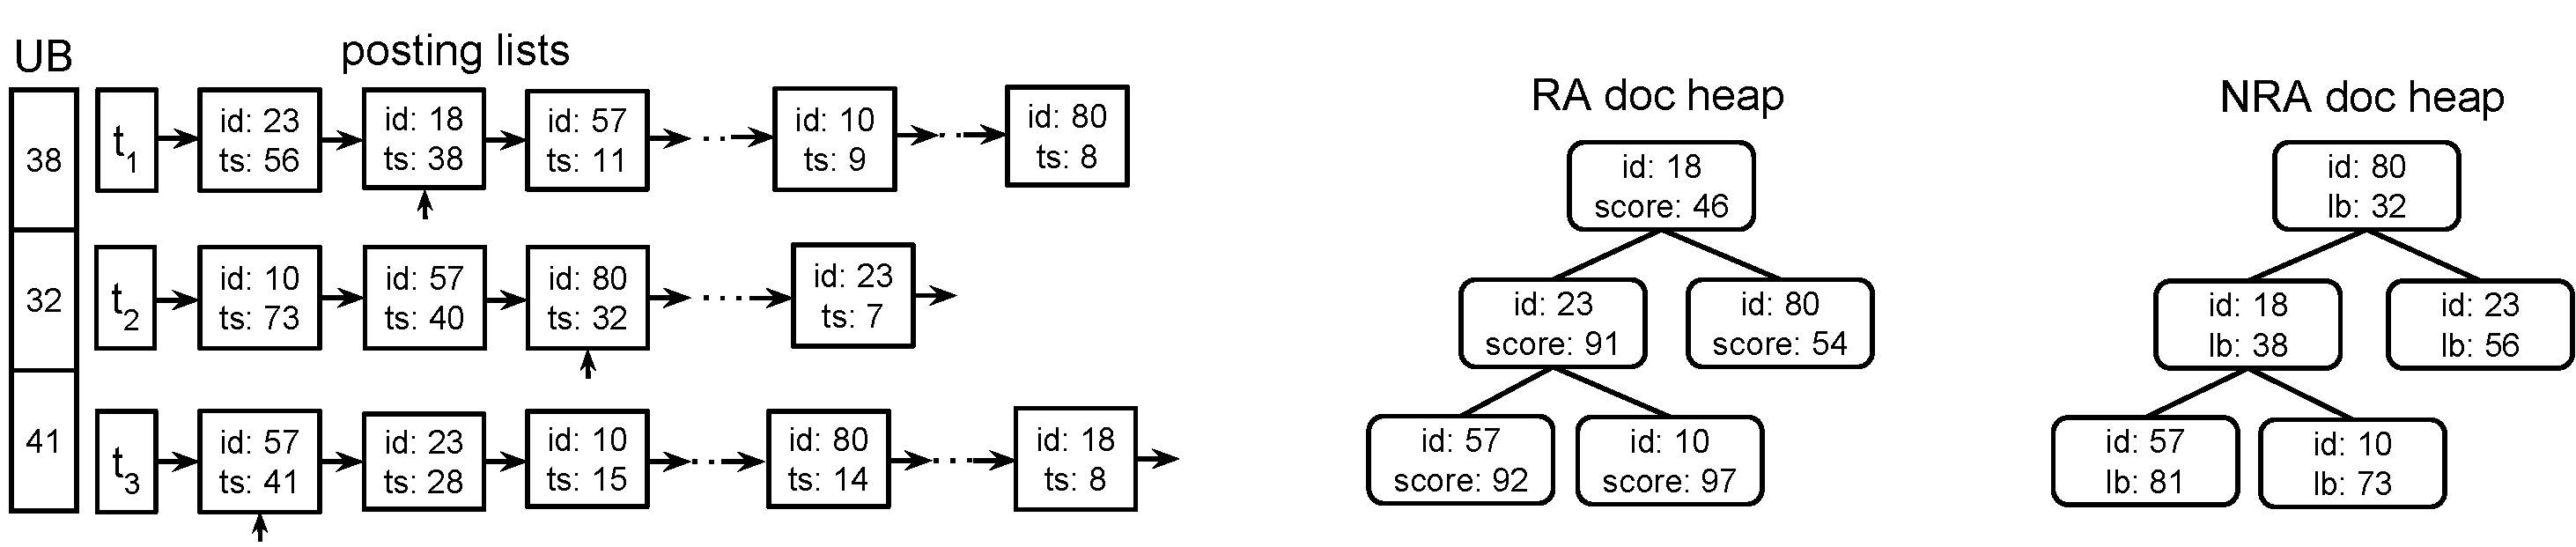
\includegraphics[width=0.95\linewidth]{figures/postingsLists}
\caption{Traversal example in  RA and NRA variants of the Threshold Algorithm (TA). Posting lists are sorted by decreasing term score. Vertical arrows depict  iterator positions.  UB  holds upper bounds on the terms' contributions to scores of untraversed documents. The RA document heap is ordered by full document score, and the NRA heap  by partial score (lower bound).}
\label{fig:lists}
\end{figure*}

%Additionally, and similarly to DAAT-based algorithms, 
TA also maintains a threshold $\Theta$, i.e., the score of the $k$-th document in the heap.
%DC, and an upper bound on all other candidate scores not yet encountered. 
It stops when no candidate can exceed the threshold score. 
Fagin et al.\ present two flavors of the algorithm, which we now describe.
%The algorithm comes in two flavors.

\paragraph{Random Access (RA)} 
The RA variant assumes that given a document id, we can use random access in order to obtain all its term scores in order to compute its total score. It thus computes the full score for every document it encounters. If the score is higher than the threshold, it is inserted into the heap. Then, $\Theta$ and the corresponding term's UB are updated. The algorithm stops when 
the following \emph{upper bound stopping condition} holds:
\begin{equation} \label{eq:stop}
\RAStop \triangleq \sum_{i=1}^m UB[i] \le \Theta.
\end{equation}

At this point, no non-traversed document can achieve a high enough score to be included in the heap. RA's output is the set of documents in the heap, ordered by their scores.

%RA is an exact  algorithm as it returns the top-k results. 
In our evaluation, we implement an approximate variant of RA by stopping whenever the heap does not change for some parameter $\Delta$ ms. 
Note that being a score-order algorithm,  TA is amenable to such early stopping: high scoring documents are likely to be discovered early.
%, and finding new high scoring documents becomes less and less likely as the algorithm progresses. 
This is in contrast with document-order algorithms, where finding high scoring documents remains equally likely throughout the execution.

\remove{
RA was shown to be \emph{instance-optimal} in~\cite{Fagin:2003}, namely, the number of times it accesses data items is asymptotically close the optimum for every problem instance. Nevertheless, this analysis assumes that all accesses to data items have the same cost. 
This assumption holds if full scoring information about all data items is available in RAM (and resides in cache), but does not hold  for big datasets. 
}
%that do not fit into RAM (at least as long as non-volatile storage hardware does not provide memory-speed random access).
Unfortunately, random access is costly,  in particular for large data sets that do not reside fully in RAM.
Whereas a sequential posting list traversal requires infrequent I/O (at the end of each data block) and exhibits cache-friendly locality of access,  each random document access entails an I/O request and a cache miss.  
An additional drawback is RA is the need to maintain a secondary index by document id in addition to the one sorted by term score, which doubles its footprint. 

\paragraph{No Random Access (NRA)} 
The alternative NRA method %scans the posting lists sequentially in an interleaved manner while avoiding random access. It
refrains from computing the full score for each traversed document, and instead
maintains lower and upper bounds for candidate documents based on {\em partially\/} computed scores. 
%DC It stops when the lower bound $\Theta$ on all candidates in the top-k heap is larger than the upper bounds of all other potential candidates. 
%In more detail, 
%NRA tracks the partial scores of the documents it encounters in the course of its traversal. 
For a document $D$ and a term $t_i$, we define the upper bound $UB(D, t_i)$ to be the term score $ts(D, t_i)$ if it has already been encountered, and otherwise $UB[i]$, which provides an upper bound on $t_i$'s term score. We similarly define its lower bound $LB(D, t_i)$ to be the term score if it is known, and zero otherwise. We then aggregate these scores to compute the document's upper and lower bounds:
\[
UB(D) \triangleq \sum_{i=1}^m UB(D, t_i) \ ; \  
LB(D) \triangleq \sum_{i=1}^m LB(D, t_i).
\] 
In Figure~\ref{fig:lists}, $UB(D_{57}) = 38+40+41 = 119$ and $LB(D_{57}) = 40+41 = 81$, whereas its actual score  is $11+ 40+41 = 92$.

NRA maintains the top-k heap according to the document \emph{lower bounds}, and $\Theta$ holds the smallest value among them. 
Its output is the set of documents in the heap, sorted by LB.

NRA's safe variant stops when (1) the \RAStop\ stopping condition of RA holds, 
and (2) all the  visited documents that are not in the heap have \emph{upper bounds} lower than or equal to $\Theta$. These two conditions are complementary: (1) ensures that no non-traversed documents are among the final top-k, whereas (2) ensures the same for  traversed documents that are not among the current top-k. 
While NRA does return the exact top-k results, unlike RA, it does not necessarily preserve the order among them, since some returned documents may be partially scored. As in RA, the approximate variant  stops after the heap has not changed for $\Delta$ ms.


\section{\alg\ }
\label{sec:alg}

\alg\/ is a parallel algorithm that applies the NRA design principles to shared-memory multiprocessor hardware platforms. 
Like our implementation of RA and NRA described above, 
it can be configured to provide approximate results by stopping after the heap does not change for some $\Delta$ time. 
\remove{
Section~\ref{sssec:ds} describes the algorithm's data
structures. Section~\ref{sssec:tasks} explains how we divide the work involved in query processing among threads. Section~\ref{sec:synch} describes synchronization around the shared data structures.
%Finally, Section~\ref{ssec:unsafe} describes the early-stopping (unsafe) version of \alg, which trades latency for recall. 
}

\subsection{\alg\ Data Structures}
\label{sssec:ds}

\begin{table}[htb]
\centering
\begin{tabular}{l l }
\hline
name & value \\
\hline
 \Docobj\ & $\langle$ int id, int score[$m$], int LB $\rangle$ \\
 \DHeap & init empty \\
 $\Theta$ & init $0$  \\
 $UB[m]$ & init $\infty$ \\
 \RAStop&  $\sum_{i=1}^m UB[i] \le \Theta$ \\
 $UB(doc)$ & $\sum_{i=1}^m \big( doc.score[i] > 0$ $?$ $doc.score[i] : UB[i] \big)$  \\
 \DMap & init empty  \\
 \HeapUpdateTime & init now \\
 \Done & init false \\
 \TMap[m] & init pointer to \DMap \\ 
  \LDMap & init empty \\ 
  \hline
\end{tabular}
\caption{\alg's data structures and  initial values.\vspace{-5mm}}
\label{alg:sparta-ds}
\end{table}

\remove{

\begin{table*}[tb]
\centering
\begin{tabular}{l l l}
\hline
name & value & description\\
\hline
 \Docobj\ & $\langle$ int id, int score[$m$], int LB $\rangle$ & document object\\
 \DHeap & init empty &  heap of \Docobj\ sorted by LB \\
 $\Theta$ & init $0$  & minimal value in $\DHeap$\\
 $UB[m]$ & init $\infty$ & upper bounds on untraversed docs\\
 \RAStop&  $\sum_{i=1}^m UB[i] \le \Theta$ & UB stopping condition\\
 $UB(doc)$ & $\sum_{i=1}^m \big( doc.score[i] > 0$ $?$ $doc.score[i] : UB[i] \big)$ & document score upper bound \\
 \DMap & init empty & maps document id to \Docobj \\
 \HeapUpdateTime & init now & time of last heap update\\
 \Done & init false & termination indication\\
 \TMap[m] & init pointer to \DMap &  per-term partial copies of \DMap\\ 
  \LDMap & init empty & temporary \DMap\ for maintenance\\ 
  \hline
\end{tabular}
\caption{\alg's data structures and  initial values.}
\label{alg:sparta-ds}
\end{table*}

}

Table~\ref{alg:sparta-ds} defines the data structures used by \alg.
%and Figure~\ref{fig:sparta_ds} illustrates them. 
As in NRA, the algorithm maintains the current top-k results in a heap, \DHeap, and its lowest value in $\Theta$. It keeps $m$ pointers to the next elements to traverse in all posting lists (not listed in Table~\ref{alg:sparta-ds})
and an array $UB$ of upper bounds on non-traversed term scores. 
$UB$ is used for computing the documents' upper bounds 
as well as for checking NRA's  stopping conditions.   

The hash map 
\DMap\ maps  document ids encountered thus far to document \Docobj\ objects. A \Docobj\ holds a vector of term scores observed thus far for this document as well as a lower bound on the document score computed as their sum.
%\DMap\ is used to maintain the partial document scores. 
NRA's first stopping condition is checked by the macro \RAStop, and the 
second stopping condition is checked as follows: 
\begin{equation} \label{eq:stop2}
\forall D\in \DMap \setminus \DHeap : UB(D) \le \Theta.
\end{equation}
The stopping conditions are evaluated by a \emph{cleaner} task,
which also checks the heap's latest update time \HeapUpdateTime\ and 
sets the \Done\ flag once the algorithm can stop.

\remove{
\begin{figure}[tbh]
\centering
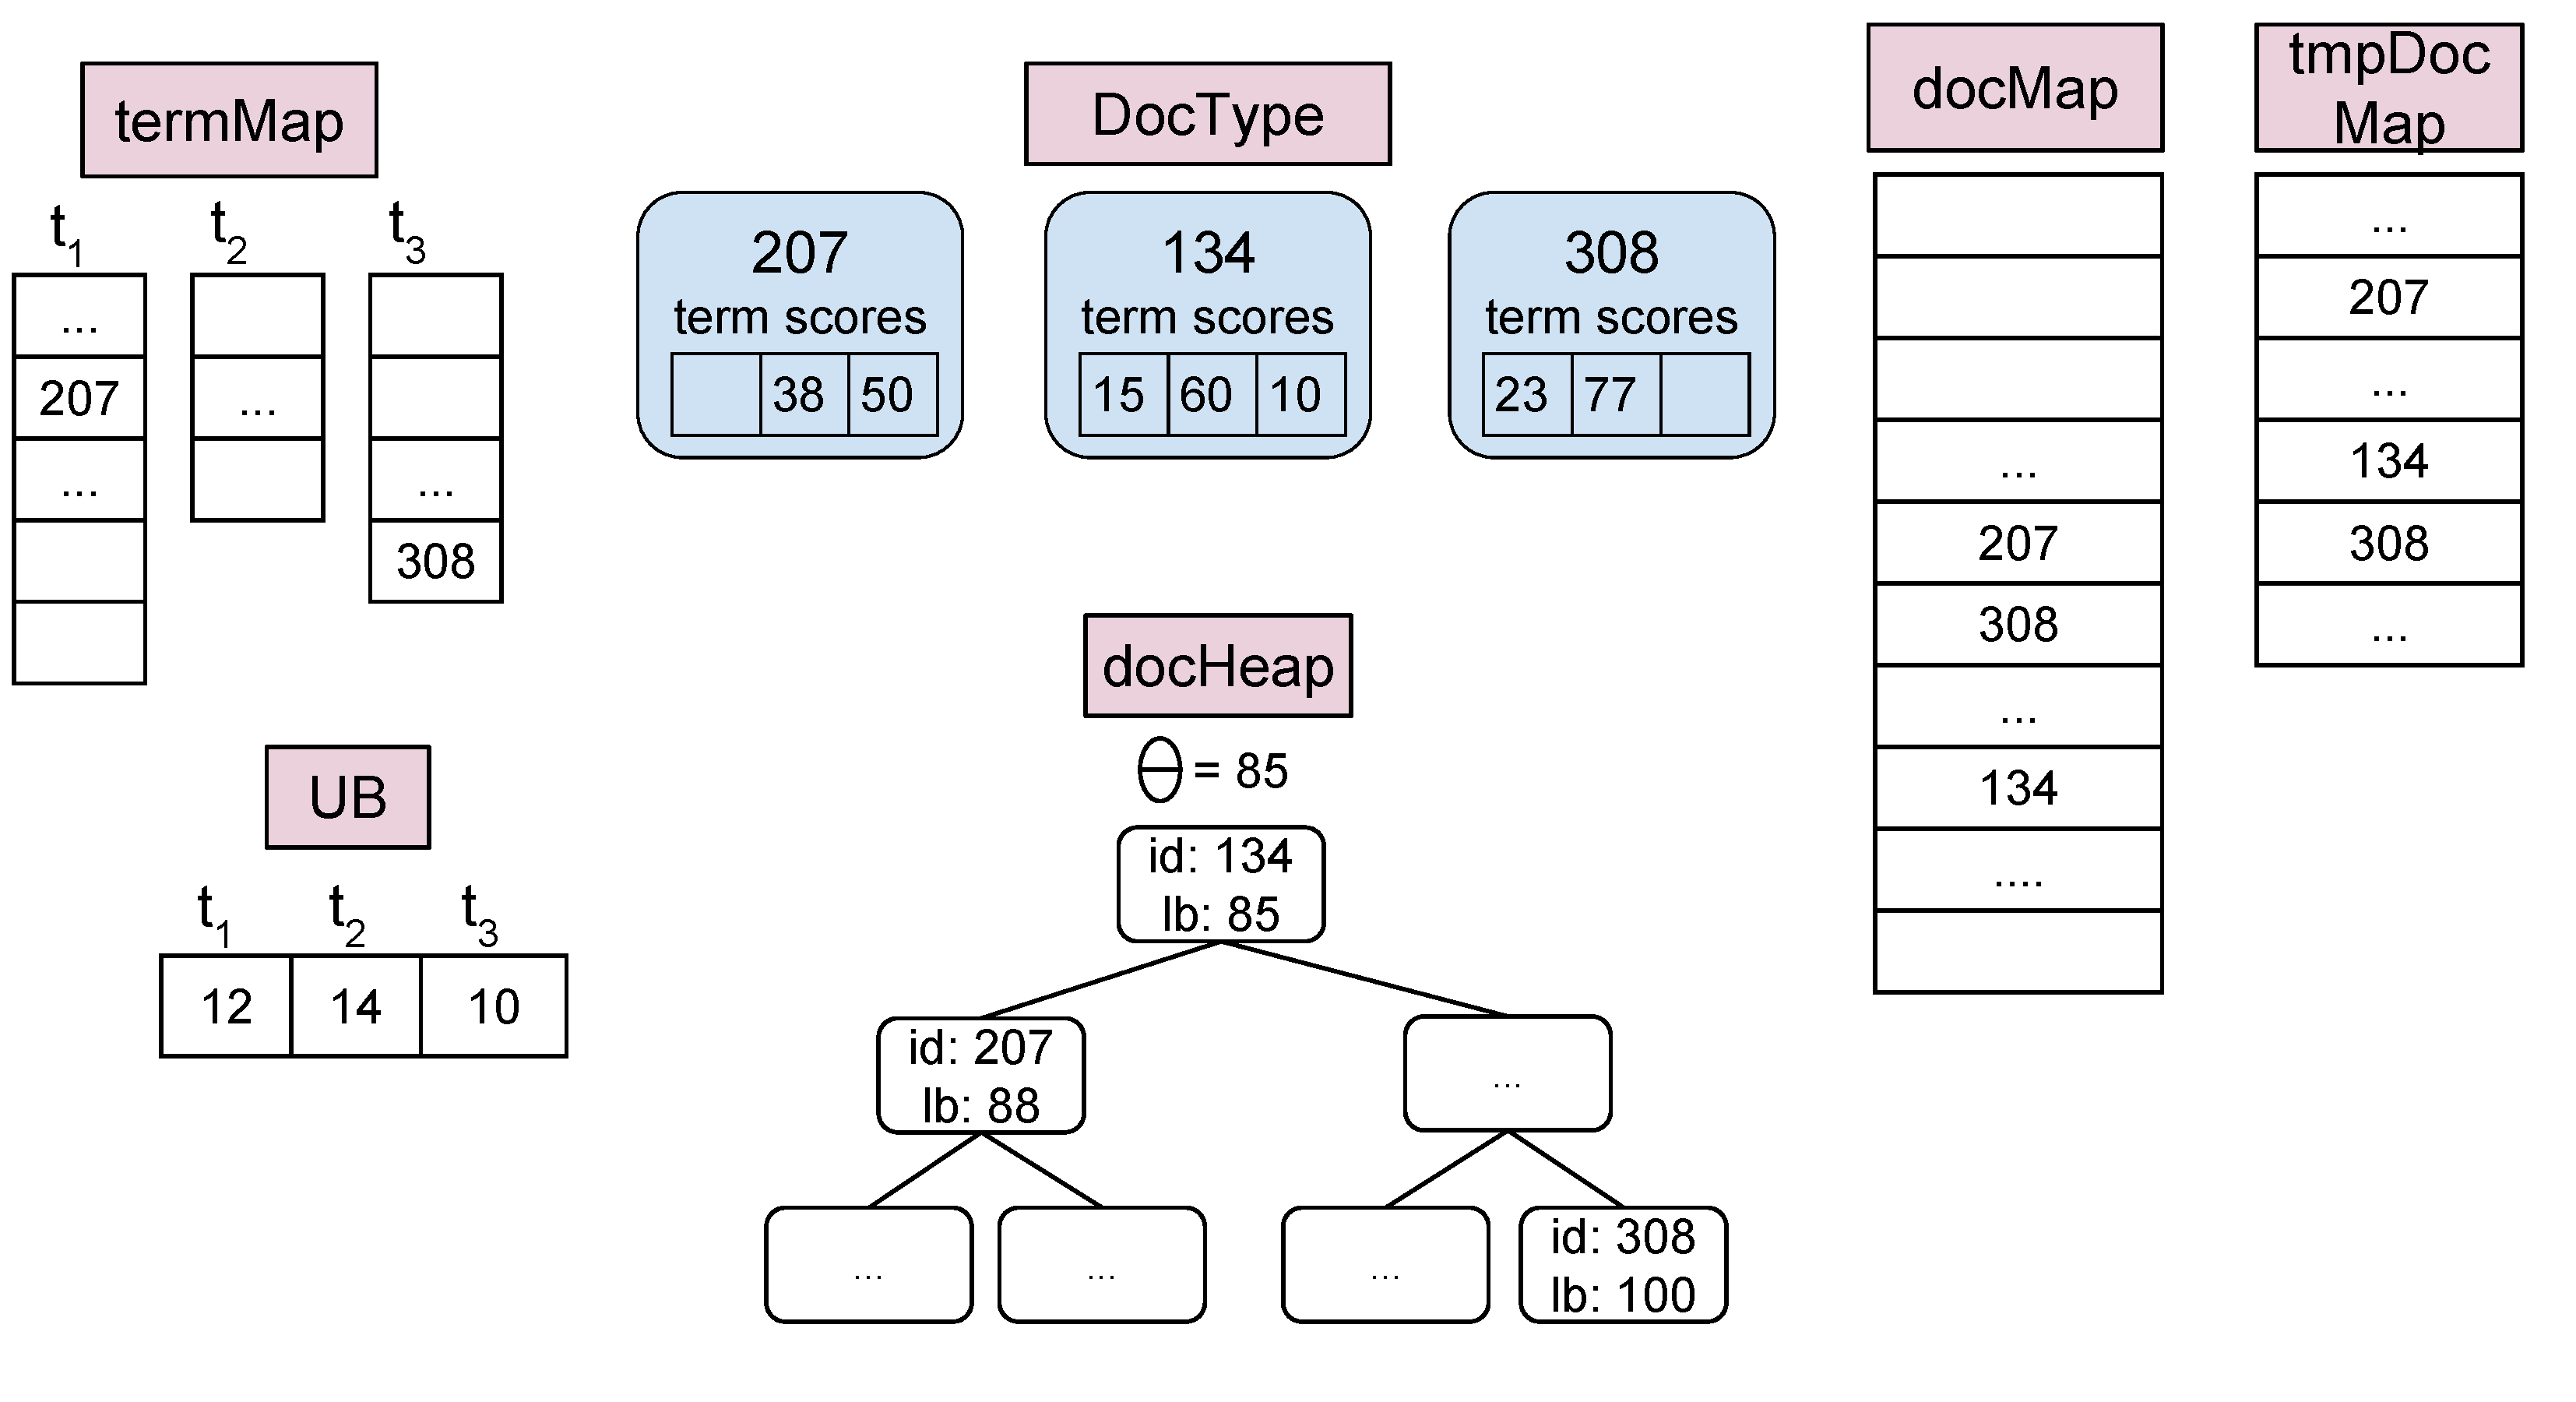
\includegraphics[width=\columnwidth]{figures/localData}
\caption{\alg\/ data structures. The \DMap\ keeps track of partially scored documents; \LDMap\ and \TMap\ are local partial copies of \DMap.}
\label{fig:sparta_ds}
\end{figure}
}

In addition, to reduce the synchronization overhead and improve cache locality, \alg\ uses 
two local data structures that hold partial copies of the global \DMap, namely the \TMap\ array with a (local) hash map per term, 
and the \LDMap\ used by a dedicated maintenance thread. The role of these will become evident 
when we discuss synchronization and locality below.

\subsection{Splitting the Work}
\label{sssec:tasks}

%Executing NRA on a multi-term query sequentially can take a long time. We shorten this time by processing queries in multiple threads running in parallel. 

A na\"ive attempt to parallelize NRA would be to 
%assign a thread per term and 
share the data structures among all threads. (Note that sharing state is essential because the partial document scores, and consequently the lower bounds, are affected by multiple threads that generate term scores). This approach 
\remove{
suffers from multiple drawbacks. For one, it requires a predefined number of threads, while a server running many queries may not always have the required number of threads available. More importantly, straightforward sharing 
}
leads to high contention, primarily around $\DMap$.%, even when the implementation uses a state-of-the-art concurrent hash map\footnote{\small{\url{https://docs.oracle.com/javase/7/docs/api/java/util/concurrent/ConcurrentHashMap.html}}}. 
%This results in even poorer performance than the sequential execution.\inred{we need to justify it}
% (see Section~\ref{sec:eval}).   

%Instead, we redesign the algorithm flow in a way that reduces contention. 
To reduce contention, we 
consider the point in time when the first stopping condition (Equation~\ref{eq:stop}) holds. From this time on, no new document's score can surpass the lower bound of any document in the shared \DHeap. Therefore, adding new documents to \DMap\ is no longer helpful (a similar observation was made  in~\cite{Mamoulis:2007}). 
On the other hand, it is possible to shrink \DMap\ by removing documents whose upper bounds are smaller than $\Theta$.
This is cardinal for the concurrent implementation, which can stop sharing \DMap\ among the threads once it is sufficiently small, thereby eliminating the synchronization overhead. 




\begin{algorithm*}[htb]
\small
\begin{multicols}{2}
\begin{algorithmic}[1]
\For{$i=1$ to $m$} \Comment processing $m$-term query
\State add {\sc processTerm($i$)} to job queue \label{l:par-init-job}
%\State \TMap[i] $\leftarrow$ pointer to \DMap
\EndFor
\State spawn up to $m$ execution threads to run jobs from queue\label{l:start-threads}
\State wait until \RAStop
%\State	
	\Comment all candidate documents are in \DMap
\State add {\sc cleaner()} to job queue %\Comment parallel with term processing
\State wait until $done$
\State return \DHeap \label{l:par-end}
%

\Statex 
\Procedure{processTerm}{$i$} 
%\Statex
%	\State $\langle id,$ score$\rangle \leftarrow$ next entry in $i$th posting list
%  	\If{$id \not\in \DMap$}
%    	\State create new document object $D$
 %       \State add $D$ to $\DMap(id)$
%	\Else 
 %   	\State $D \leftarrow \DMap(id)$
%	\EndIf
%	\State {\sc evaluate}($D$, score, $i$)
 %   \State $UB[i] \leftarrow$ score 
  % 	\Comment update term's upper bound \label{l:seq-update-ub}
%\EndIf
%\Statex 
	\If{\RAStop\, $\wedge\, |\DMap | < \Phi $}  
		\Comment \DMap\ is shrinking and small
		\If{\TMap[i]=\DMap} \label{l:hash-start}
		\State {\sc initMap($i$)}
  	\EndIf \EndIf \label{l:hash-end}
%    \Statex
	\For{$j=1$ to \emph{segSize}} 
%	\Statex \Comment evaluate documents in segment
		\If{\emph{done}} return \EndIf
    		\State $\langle id,$ score$\rangle \leftarrow$ next entry in $i$th posting list
		\State $D \leftarrow$ \TMap$[i](id)$
 	  		\If{$D = \bot$} \Comment document missing 
 	  			\If{$\neg$\RAStop} \Comment hash incomplete
		 			\State create new document object $D$
 					\State add $D$ to $\TMap[i](id)$
				\Else\ continue
				\EndIf
    			\EndIf
        			\State $D.score[i] \leftarrow$ score \Comment update $D$'s term $t_i$ score
			\If{$\Sigma_{j=1}^{m} D.score[j] >  \Theta$}  
			\Comment $D$ belongs in heap
				\State {\sc update\_heap}($D$)
			\EndIf	
	\EndFor % $id$ is last in chunk
	\State $UB[i] \leftarrow$ score \Comment update term's upper bound \label{l:thread-update-ub}    
	\State add {\sc processTerm($i$)} to job queue \label{l:new-task}
\EndProcedure

%\Statex

\Procedure{initMap}{$i$}	
        			\Comment create cache-friendly local copy of \DMap\ %for evaluating term $i$
        			\State \TMap[i] $\leftarrow$ new hash map
    			\ForAll{$D \in$ \DMap\ where $D.score[i] = 0$} 
            			\State add $D$ to \TMap[i] \label{l:hash-chash}
            		\EndFor
\EndProcedure
\Statex 
\Procedure{update\_heap}{$D$} 
\State lock \DHeap \label{l:lock-heap}
\If{$D\not\in$\DHeap} 
	\State insert $D$ to \DHeap
	\ForAll{$d \in$ \DHeap}  \label{l:for-all-heap-docs}
		\State $d$.LB $\leftarrow \Sigma_{j=1}^{m} d.score[j]$
		\State move $d$ to correct place in heap \label{l:fix-heap}
	\EndFor
	\If{$|\DHeap | > k $} 
		\State remove doc with the lowest score from \DHeap
	\EndIf
	\If{$|\DHeap | = k $}
		\State  $\Theta \leftarrow$ lowest score in \DHeap
	\EndIf
	\State \emph{HeapUpdateTime} $\leftarrow$ current time 
\EndIf
\State unlock \DHeap  \label{l:unlock-heap}
\EndProcedure
%
%
\Statex 
\Procedure{cleaner}{} \label{l:clean-start}
%\While{\DMap\ has more than $k$ entries}
\If{$|\DMap | > \Phi $} 
\State \LDMap\ $\leftarrow$ new hash map \label{l:clean-local-copy}
%a local copy of \DMap 
\For{every doc $D$ $\in$ \DMap} 
\If{$UB(D) > \Theta \vee D \in$ \DHeap}
	\State add   $D$ to \LDMap
\EndIf
\EndFor
\State replace \DMap\ by \LDMap \label{l:clean-replace}
\EndIf
%\Statex
%\State \emph{Stop} $\leftarrow \big( |\DMap| = |\DHeap| \big)$ 
\If{\emph{HeapUpdateTime} $ + \Delta < $ now $\vee\ \big( |\DMap| = |\DHeap| \big)$ } \label{l:clean-stop-cond}
\State \emph{done} $\leftarrow$ true
\Else\ add {\sc cleaner()} to job queue
\EndIf
\label{l:clean-end}
%\EndWhile
\EndProcedure 
\end{algorithmic}
\end{multicols}
\caption{\alg\ algorithm.}
\label{alg:sparta}
\end{algorithm*}

The algorithm's pseudocode appears in Algorithm~\ref{alg:sparta}. It 
exploits up to $m$ {\em worker\/} threads per query, but can run with fewer threads if less are available. 
We divide posting list traversals to segments of size \emph{segSize}, and use a job queue to allocate posting list segments to threads (line \ref{l:par-init-job}). 
The  {\sc processTerm($i$)} function processes the next segment of term $t_i$. 
A  thread that finishes its assigned segment inserts into the queue a new task for scanning the next segment in the same term's posting list 
(line~\ref{l:new-task}). Thus, we  progress on all posting lists at the same rate modulo the segment size. 
In case $m$ threads are available, a large segment size can be used.

In addition to  posting list-traversing tasks, the 
{\sc cleaner} function (lines~\ref{l:clean-start}--~\ref{l:clean-end}) performs maintenance on the \DMap.
This task is invoked once Equation~\ref{eq:stop} holds and so  \DMap\ no longer grows.
The cleaner serves two purposes. First, as its name suggests, it removes 
entries that ceased to be top-k candidates from \DMap. %, thus reducing its size.  
Since \alg\ is memory-intensive, a smaller \DMap\  allows it to run much faster; 
(a similar observation, in a sequential setting, was made in~\cite{Gursky:2008}). 
Second, it detects the stopping conditions (line \ref{l:clean-stop-cond}). In the approximate version, it checks whether the heap has not changed for $\Delta$ time 
(the exact version is obtained by setting $\Delta=\infty$). It also checks the  condition of Equation~\ref{eq:stop2}: 
once \DMap\ is the same size as \DHeap\ we know that the two are identical because \DMap\ always includes all \DHeap\ entries. 
At this point, \DHeap\ holds the top-k scored results, and stopping is safe. 
%
Once the algorithm stops, the main thread returns the heap's contents. 

\subsection{Synchronization} 
\label{sec:synch}

Note that, \DHeap, $UB$, \DMap, and \Docobj\ objects referenced by them are accessed concurrently by multiple threads. We need to protect such access to avoid inconsistencies. On the other hand, reducing contention is crucial for performance. Moreover, 
\alg\ is a memory-intensive algorithm, and 
%primarily with respect to the shared \DMap. During the parallel phase, multiple threads access it frequently, for reading. 
in order to keep the memory access latencies low, it is paramount to exploit the CPU hardware cache, in particular the core-private L1 caches. 
We now explain how we synchronize access to each of the shared variables
in a way that reduces contention and improves cache utilization. 



Since at most one thread processes each term, no races arise around updating $UB$ entries, and no lock is needed. However, 
all threads read all $UB$ entries, and therefore frequent updates can lead to frequent cache misses, and in turn, poor performance. 
%Note that during the sequential phase, the UB array is updated after each partial document evaluation (line \ref{l:seq-update-ub}), which occurs frequently.
In order to reduce the number of cache misses, instead of updating $UB$ after each document evaluation, the workers update it lazily, at the end of a segment traversal (line \ref{l:thread-update-ub}). Since upper bounds can only decrease whereas $\Theta$ can only increase, such lazy updates do not affect correctness.

%while speeding up the execution.
Updates of \DHeap\ and $\Theta$ are protected by a shared lock (lines~\ref{l:lock-heap} and~\ref{l:unlock-heap}), which  serializes all updates. 
%However, since most heap updates occur in the sequential phase, parallel updates are infrequent, and this does not constitute a performance bottleneck. 
To avoid races around evaluating a \Docobj's
lower bound and inserting it into \DHeap, we update the lower bound in a lazy manner while holding the global lock on \DHeap: Every thread that adds a document to the heap updates the lower bounds of all heap documents (lines \ref{l:for-all-heap-docs}-\ref{l:fix-heap}).

Before the first stopping condition (Equation~\ref{eq:stop}) holds, multiple workers update \DMap\/ concurrently. 
We therefore protected each hash bucket by a granular lock, which  
performed better than the generic Java concurrent hashmap\footnote{\small{\url{https://docs.oracle.com/javase/7/docs/api/java/util/concurrent/ConcurrentHashMap.html}}}.

The cleaner task starts removing elements from  \DMap\/ after it is guaranteed that 
no new entries are added to  it; such removals substantially improve the term processing performance. 
Nevertheless, allowing the cleaner to constantly update \DMap\ would lead to frequent cache invalidations at the
tasks that read the map. 
To avoid frequent cache misses, 
%such frequent synchronization between the cleaner and term-processing tasks, 
the global map is kept read-only most of the time, while the cleaner works on a local copy: 
it  
%Specifically, as long as its stopping condition is not satisfied, 
%the cleaner 
repeatedly builds a new map \LDMap, holding \DMap\ entries whose upper bounds 
are higher than $\Theta$ as well as ones that are included in \DHeap\ (whose upper bounds may be exactly $\Theta$); recall that other \DMap\ entries no longer need to be kept. 
Once \LDMap\ is ready, the cleaner replaces \DMap\ with it via a single pointer swing 
(flipping the global reference). 

%\subsection{Locality Optimizations}
%\label{sssec:locality}

%\alg\/ is a memory-intensive algorithm, primarily with respect to the shared \DMap. During the parallel phase, multiple threads access it frequently, for reading. In order to keep the memory access latencies low, it is paramount to exploit the CPU hardware cache, in particular the core-private L1 caches. 

%We call this concurrent algorithm SharedState. SharedState runs much faster than the sequential NRA, and scales to very long queries. We now proceed to the full version of \alg, which further improves the performance. \inred{Gali: the full version only adds the local hash maps, so maybe we should present it in a different way. We also don't have to present SharedState here, it can be done in the evaluation section}

Access to \DMap\ is a principal performance bottleneck, since it is frequently read by all worker threads. Initially, it is too large to fit into local caches, and so the parallel execution inherently requires global memory accesses. But thanks to the cleaner's work, \DMap\ shrinks in the course of the execution. 
Moreover, not all  \DMap\ entries are relevant for all terms -- if $D$'s term score for $t_i$ has already been computed, then a  thread handling term $t_i$ does not need to access $D$.
Thus, the relevant subset of  \DMap\ for each term eventually becomes small enough to fit in its local cache. As long as the thread continues to access the global \DMap,  it  experiences massive cache misses every time the cleaner replaces the global \DMap. 
%As long as $\DMap$ is big, it is more important to shrink it fast than avoid those misses. However, 
But 
once it becomes small enough to fully fit in the local cache, there is no need to keep using the global copy. 

To this end, \alg\/ associates a local map replica, \TMap, with each posting list. \TMap\ is created by the worker that currently owns that posting list once \DMap's size drops below a threshold $\Phi$,
in our implementation, $\Phi=10$K entries. The {\sc initMap} function scans \DMap, and copies to \TMap\ the references to those \Docobj{} objects that do not contain the score for the worker's term yet.  Once a \TMap\ has been created, every worker that handles its posting list uses it.
Note that since every posting list is accessed by a single worker at any given time, no synchronization is required.
%
%We show in the next section that by using \TMap s, we expedite \alg's query processing latency by up to $35\%$.

\subsection{Analysis}

\alg\ accesses posting lists in the same manner as NRA does, and stops only when NRA's stopping conditions hold. Thus, like NRA, its 
exact version ($\Delta = \infty$) is safe, and returns the top-k results. 

In terms of performance, NRA was shown to be \emph{instance-optimal} when  random access is impossible~\cite{Fagin:2001}, 
namely, its number of accesses to posting list entries is asymptotically close the optimum for every problem instance.  
This property holds for pNRA as long as the rates in which different threads access different posting lists are within constant multiples of each other~\cite{Fagin:2001}, because in this case a thread that ``runs ahead'' without knowing it should stop only accesses a constant factor more entries than the algorithm needs to, which the asymptotic
analysis ignores. \alg\ differs from pNRA in delaying updates to UB until the end of the segment, 
which may further delay stopping until the thread accesses \emph{segSize} posting list entries. Since \emph{segSize} is constant, \alg\ is asymptotically
instance-optimal under the same assumptions as pNRA.



\section{Case Study: Web Search} \label{sec:eval}

We conduct a case study of top-k query processing on a web dataset. 
We compare the performance of \alg\ to the following multiprocessor algorithms: 
%\inred{
\begin{description}
\item[\pBMW]\cite{rojas2013efficient} -- parallel BMW,  
the best-in-class parallelization of a document-order top-k algorithm; 
\item[\pJASS]\cite{parallel-jass} -- a recent parallelization of the JASS~\cite{Lin:2015} score-order retrieval algorithm; 
\item[\pRA]-- a parallel implementation of RA;
\item[\sNRA]--  a shared-nothing  parallelization of NRA; and 
\item [\pNRA]-- a
na\"{\i}ve shared-state parallel implementation of NRA. 
\end{description}
%}
%Although our primary focus is   approximate top-k, for completeness, we also experiment with the algorithms' exact variants.



In order to crystallize the comparison among  the core algorithms, 
we abstract away other contributors to the wall-clock  latency, e.g., index compression. 
As recent studies show, given state-of-the-art compression techniques, the impact 
of decompression on end-to-end performance is marginal (e.g., up to $6\%$ with QMX-D4 compression~\cite{Lin:2017}).  
%Compression effectiveness of document-order vs score-order indexes is beyond the context of this paper.

We focus on disk-resident search indexes. 
%(most of the algorithms under study are of streaming nature, and hence CPU-bound; fitting the index in RAM does not affect their performance significantly). 
We also experimented with RAM-resident indexes, and in all cases, all algorithms except \pRA\ got similar results, which is not surprising given that the algorithms traverse posting lists sequentially. These results are omitted for lack of space.

\remove{
In what follows, Section~\ref{ssec:setup} describes the experiment setup, 
Section~\ref{ssec:implementation} explains how the algorithms are 
implemented, and Section~\ref{ssec:results} presents our results.
}

\subsection{Methodology}
\label{ssec:setup}

We study  algorithms in terms of query latency and throughput attainable at a single multi-core server. 
We use mid-tier industry-standard hardware -- a 12-core Intel Xeon E5620 with 24GB RAM and 1TB SSD drive. 

The benchmarking environment and the algorithms  are implemented in Java. 
A  {benchmark driver} draws queries from an input queue and submits them to the algorithm being tested, which
% It runs the queries either one-by-one (latency mode) or in parallel (throughput mode). 
%In both modes, the algorithm  
uses a thread pool for intra-query parallelism. 
The driver controls the pool size. % by notifying the algorithm how many threads are available to it.
When testing latency, the entire thread pool is used by a single query. 
In the throughput evaluation mode, queries are scheduled first-come-first-served, 
and a new query is scheduled for execution (i.e., assigned threads) 
once  there are idle threads with no outstanding work from currently executing queries.
All queries scheduled for execution equally share the thread pool.

In all experiments, the appropriate index (either in document order or in score order)
is pre-built offline and stored on disk uncompressed as a collection of binary files, 
each storing a shard of data partitioned by term.  The benchmark environment memory-maps the contents 
of these files via the MappedByteBuffer API~\cite{java-bytebuffer}.
Prior to each experiment, we flush the file system's page cache so all pages are physically read from disk during the experiment.


%such that the algorithm code can access the data identically to RAM. 
%The application code makes no attempt to optimize the disk access beyond the standard filesystem mechanisms 
%(e.g., caching of popular blocks). 

%\subsubsection{Datasets}
We  experiment with two document corpora. The first  is 
the TREC dataset, Category B ({\cw}09B), which is widely used for information retrieval research~\cite{ClueWeb09}. This dataset includes approximately 50M web documents and takes up roughly 30GB of original content, uncompressed.


The second corpus is a synthetic 10x scale-up of \cw, named \cwten, which we created to explore the algorithms' scalability 
with the dataset size. 
% \cwten\ is a superset of {\cw}09B.
The 450M synthetic documents in {\cwten\/} are generated as follows. Each document is a bag of words drawn from the original {\cw\/} dictionary 
(the order is immaterial for our document scoring function) 
%, see Section~\ref{ssec:scoring}) 
so that the number of occurrences of a term $t_i$ with an original 
global frequency rate of $F(t_i)$ is drawn from a geometric distribution with a stopping probability of $1-F(t_i)$. This  process preserves 
the  term frequency distribution of {\cw\/} in \cwten.

 
We use the popular Lucene open-source search engine~\cite{lucene} for preprocessing the index to generate posting lists; this  includes text tokenization, posting list maintenance, 
and term statistics retrieval.
We score documents using a standard tf-idf score function with document length normalization~\cite{Baeza-Yates:1999:MIR:553876}. 

We draw queries from the public AOL search log~\cite{aol}.
For each number of terms from $1$ to $12$, we independently sample $100$ queries of this length uniformly at random from the AOL log.
We also  experimented with a query log of another commercial web search engine; this experiment  
produced statistically similar results, and so we omit them here.  

We use  $k=1000$, {based on the assumption that simple tf-idf retrieval is the first phase of multi-stage ranking, 
which may require large values of $k$ for effectiveness~\cite{Wang:2011}. (Indeed, Crane et al.~\cite{Crane:2017} report
that the classical AP and RBP quality metrics are close to optimal with this choice of $k$, for multiple datasets.)
Experiments with $k=100$ produced qualitatively similar results, which we omit for lack of space.

\remove{
\subsubsection{Document Scoring}
\label{ssec:scoring}
For document evaluation, we apply a simple tf-idf score function with document length normalization~\cite{Baeza-Yates:1999:MIR:553876} as follows:
\[ \textit{ts}(D, t_i) \triangleq \frac{\textit{idf}(t_i) \cdot \textit{freq}(D, t_i)}{\sqrt{|D|}},\]
where \textit{freq}$(D, t_i)$ is the frequency of term $t_i$ in document $D$,
$\textit{idf}(t_i)$ is  the inverse document frequency of term $t_i$,
and $|D|$ is the number of tokens in $D$. 
}

\subsection{Implementation}
\label{ssec:implementation}

%All algorithms store 
Posting lists are stored as contiguous uncompressed arrays;  {\pRA} also stores 
its secondary index (document id to position in the posting list mapping) in the same form. 
Term scores (namely, tf-idf) are stored in the posting lists as integers, scaled by $10^6$ and rounded as in~\cite{Bortnikov:2017}. 
Using integer arithmetic instead of floating-point significantly speeds up document evaluation. 

The specific algorithm implementations are as follows.

\subsubsection{State-of-the-art parallel search algorithms}

\paragraph{\pBMW}
Our implementation of {\pBMW} closely follows the description in~\cite{rojas2013distributing}. The algorithm partitions the execution of the 
sequential BMW~\cite{Ding:2011} among multiple threads. Each thread handles a distinct subset of documents, and computes a local top-k 
result. The algorithm then merges the partial results to obtain the final top-k. 
%See Section~\ref{sec:related} for detail.

Similarly to \alg, \pBMW's threads obtain jobs from a common job queue. Here, a job defines a range of document ids to scan. 
We set the number of jobs to be twice the number of worker threads, and assign equal-size ranges to all threads.  
This partition results in well-balanced executions in which the whole worker pool is utilized 
most of the time. 

Each thread maintains a thread-local heap with the current top-k documents. (We also experimented with a shared heap and 
got inferior results; a similar finding was reported in~\cite{rojas2013distributing}.)
Similarly, each thread $T$ maintains a local threshold $\Theta_T$ for filtering heap insertions; 
$\Theta_T$ is \emph{at least} the lowest score in the local heap, but may be higher due to the progress of other threads.  
%Specifically, threads benefit from each other's progress via a shared $\Theta$ variable. 
Thread $T$ periodically compares $\Theta$ to its local $\Theta_T$ and promotes the smaller of the two to $\max(\Theta_T, \Theta)$. 
This way,  slower workers catch up with  faster ones.

\pBMW\
%, which is applied to a segment of posting lists, further 
splits posting list segments into blocks, and uses block-level
statistics to prune the search~\cite{Ding:2011}. We experimented with multiple block sizes and selected $64$, 
which yielded the best performance.
% In 
The approximate version's pruning aggressiveness is  controlled by  a parameter 
$f \geq 1$, which multiplies $\Theta$ to relax the threshold for score upper bounds~\cite{Broder:2003}. For $f=1$, the algorithm is exact.

\paragraph{\pJASS}
Our implementation of pJASS  follows the description in~\cite{parallel-jass}. It traverses all posting lists in parallel, in score order, and accumulates the encountered scores 
per-document in  \emph{docMap}. Each document is protected by a lock, and a thread that encounters a document locks it, adds the partial score from the term it traversed, and then unlocks it.
The algorithm stops after scanning a predefined fraction, $p$,  of postings. In the exact version, $p=1$.


\subsubsection{Parallel TA variants}

\paragraph{\sNRA}
\sNRA\ is a shared-nothing parallelization of NRA, where the index is partitioned to $12$ shards by document id. 
Each thread finds the top-k documents in its shard by running NRA independently with thread-local data structures. 
When all threads complete, their lists are merged and the global top-k documents are kept.  

\paragraph{\pNRA}
\pNRA\ is a na\"{\i}ve shared-state parallelization of NRA that does not employ \alg's optimizations. 
Namely, it uses a shared document map, which it does not clean, and it updates the term
upper bounds upon every document evaluation. As in \alg, a dedicated task checks the stopping condition.
(Distributed stopping detection yielded worse results).

\remove{
Similarly to {\pNRA} and \alg, {\pRA} traverses the posting lists in segments, using a job queue. 
In contrast with them, {\pRA} computes complete document scores using its secondary index, 
instead of maintaining partial scores. 
Note that {\pRA} is the only studied algorithm that exercises random access to persistent storage.  
} 

\paragraph{\pRA}
Our implementation of \pRA\ maintains its results in a shared heap (experiments did not show any benefit to using local heaps).
Note that the algorithm's multiple worker threads may encounter postings of the same document independently, 
and consequently score that document and try to insert it into the heap multiple times. The implementation 
allows only the first to take effect.

%{\pRA} halts execution if no new results have been produced for $\Delta$ time ($\Delta=\infty$ means the result is exact). 
Since RA's stopping detection is lightweight, we do not dedicate a task to it. Instead, all workers check the  
\RAStop\ condition, monitor the time elapsed since the last heap update and notify each other if they 
decide to stop.
%A thread that detects that the algorithm can stop notifies all threads.



\subsection{Results}
\label{ssec:results}

Although our focus is on approximate top-k, we experiment first with the exact variants of the algorithms. 
For an algorithm A, we denote its exact variant A\ex. We then consider approximate variants with high and low recall,
denoted  A\hi\ and A\lo, respectively. Note that the approximate algorithms' parameters ($\Delta$, $f$, and $p$) affect the recall
but do not control it directly; our high recall instances are ones that empirically achieve a  recall of $96\%$ or 
higher.
 

\remove{
We evaluate the query processing latency and throughput 
induced by the candidate algorithms, 
for $k=1000$. 
(Experiments with $k=100$ produced qualitatively similar results).
 }


\subsubsection{Exact Algorithms}

\begin{table}[tbp]
\small
\begin{center}
\begin{tabular}{l | c  c  c  c  c  c}
%\hline
   & Sparta & \pNRA & \sNRA & \pRA & \pBMW & pJASS \\ \hline
 CW & $860$ & $13\!,291$ & $5\!,553$ & $480$ & $750$ & $54\!,343$ \\ \hline
 CWX10 & $12\!,010$ & N/A & $56\!,223$ & $7\!,410$ & $10\!,210$ & N/A \\

%\hline
\end{tabular}
\end{center}
\caption{Average query latency (in ms) of 12-term queries with exact algorithms using 12  threads. 
N/A indicates the algorithm crashed due to lack of memory.
None of the algorithms meets  real-time SLAs. }
\label{tab:safe-latency}
\end{table}

Our first experiment looks into the feasibility of using exact algorithms. 
Usability studies (e.g.,~\cite{Arapakis:2014:IRL:2600428.2609627}) show that users are extremely sensitive to end-to-end delays beyond 500 ms, 
and any excess delay beyond 250 ms leads to material degradation in their experience.
Therefore, a typical  SLA (service-level agreement) for a top-k service requires queries to be served within 250 ms on average.

 Our experiment shows that none of the exact algorithms meets a real-time SLA for  long queries. 
Table~\ref{tab:safe-latency} depicts the mean processing latencies of 12-term queries with 12 worker 
threads (i.e., a single query fully exploits the multi-core CPU). 
While on \cw\ some algorithms complete within less than a second, 
on \cwten,  some algorithms crash, and others take between 7 seconds and nearly a minute, which is clearly unacceptable.

We revisit the algorithms' execution dynamics -- namely, how fast they accrue their results -- 
as we study approximate algorithms in the sequel. 
 
\subsubsection{Approximate Algorithms}
 
With  exact  algorithms failing to match  real-time requirements, we turn to focus on the approximate instances. 
We parameterize \alg, \pRA, \pNRA, and \sNRA\/ with $\Delta=10$ ms. 
This yields high recall in all four algorithms. 
We instantiate \pBMW\/ with $f=5$ for high recall and $f=10$ for low recall.  
{Finally, \pJASS\/ is instantiated with $p=0.005$ for low recall and $p=0.02$ for high recall (using $p=0.1$, as suggested, e.g., 
in~\cite{Crane:2017}, produced unacceptably high latencies).
The recall achieved with these parameters for 12-term queries is summarized in 
Table~\ref{tab:recall-mrr-distance}. 
%We see that the MRR-distance is high for the high-recall algorithms, 
%metric is closely correlated with recall 
%e.g., \alg\hi\/ yields $99\%$ recall and $0.002$ MRR-distance on \cwten. That is, these 
%algorithms not only  retain a large fraction of the true results, but also succeed in retaining the highest ranked ones. 

\remove{
This result is particularly interesting for \alg, which only computes partial scores. In practice, these scores are very close to the complete ones. 
In our experiments, on average, $93\%$ of the top-k documents have a correct score at the end of the execution. The average Pearson correlation
 between the correct scores and the partial scores is $0.999$.%, whereas the average Kendall's $\tau$ rank correlation is $0.86$. 


Summing up, under certain parameter choices the approximate algorithms achieve very high accuracy. We now focus on their performance. 
}
  
\begin{table*}[htbp]
\centering
\small
\begin{tabular}{ l | c  c  c  c  c  c  c  c }
%\hline
       &    \alg\hi &  \pRA\hi & \pNRA\hi & \sNRA\hi & \pBMW\hi & \pBMW\lo & \pJASS\hi & \pJASS\lo \\ \hline
\cw & 
   97.5\%  &  98.5\%  & 98.5\%  & 99\%   & 97.5\% & 80\%  & 96\% & 93\%
  % 97.5\% / 0.004 &  98.5\% / 0.002 & 98.5\% / 0.002 & 99\% / 0.001  & 97.5\% / 0.009 & 80\% / 0.048 
  \\ 
  %\hline
 \cwten &   99\%  & 99\%  & 99\%  & 99\%  & 97\%  & 79.9\%  & N/A & 99\%  
  \\ 
  %\hline
  % 99\% / 0.002 & 99\% / 0.001 & 99\% / 0.001 & 99\% / 0.001  & 97\% / 0.009 & 79.9\% / 0.099 
\end{tabular}
%\caption{Recall / MRR-distance induced by the approximate algorithms for 12-term queries.}
\caption{Recall of approximate algorithms for 12-term queries.}
\label{tab:recall-mrr-distance}
\end{table*}

\paragraph{Latency.}
Figures~\ref{fig:terms-scaling-high-avg}--~\ref{fig:terms-scaling-low-avg} depict the scaling of single-query latency with query length.
The number of workers in each test is equal to the number of terms (for \alg, \pRA, and \pNRA, this allows maximal parallelism). 
Figures~\ref{fig:terms-scaling-high-avg} and \ref{fig:terms-scaling-high-95} present, respectively, the  mean and  
$95\%$ latencies of queries  on  {\cw} in the high-recall algorithms. The latter captures the so-called ``tail latency'' of 
the slowest $5\%$ of the queries. 
\alg\/ outperforms all other algorithms in terms of both average latency and the 95th percentile, on all query lengths.
The margin is noticeable for long queries.

Perhaps surprisingly, although we saw (in Table~\ref{tab:safe-latency}) that  \pRA\ex\ outperforms \alg\ex,   
the trend is reversed in the approximate variants: \pRA\hi's latency for $12$-term queries it is more than $2$x slower than \alg\hi's. 
This means that \alg\/ spends much more work than \pRA\/ 
in order to collect the remaining $2.5\%$ of the exact result set. We revisit this phenomenon  below. 
While \alg\ collects the approximate results quickly, the performance of  \pRA\ suffers 
due to intensive access to the secondary index that cannot be sustained even with modern SSD hardware. 

Figure~\ref{fig:terms-scaling-10x-avg} depicts the mean latency for \cwten\ in all algorithms.
 \alg's average  latency scales perfectly, 
remaining below $180$ ms for all query lengths
 for both \cw\/ and \cwten.  
In other words, \alg's result set solidifies after processing 
a similar number of postings,  even when the overall index size grows $10$x. 
Its  $95\%$ latency is below $500$ ms. 
None of the other algorithms scales as well to the big dataset.

Figures~\ref{fig:terms-scaling-low-avg} and~\ref{fig:terms-scaling-low-95} 
compare  \alg\hi\  against the low-recall variants of state-of-the-art web algorithms. 
By sacrificing recall, \pBMW\ and \pJASS\ do improve performance and bring their tail latencies for short queries below \alg's. 
Note that this is in line with the use case for which they were developed -- predictable performance on short queries.
Yet neither algorithm is able to meet \alg's average latency for any query length or its tail latency for long queries. Moreover, 
neither algorithm fairs well on the large data set. 
For example, \pBMW\hi\/  processes 12-term queries  within $630$ ms on average on \cw, and within as long as $9.9$ seconds on \cwten. 
\pBMW\lo, which sacrifices $20\%$ of the recall for performance, only improves this latency by $15\%$.

\begin{figure*}[tbh]

      \begin{subfigure}{0.325\textwidth}
         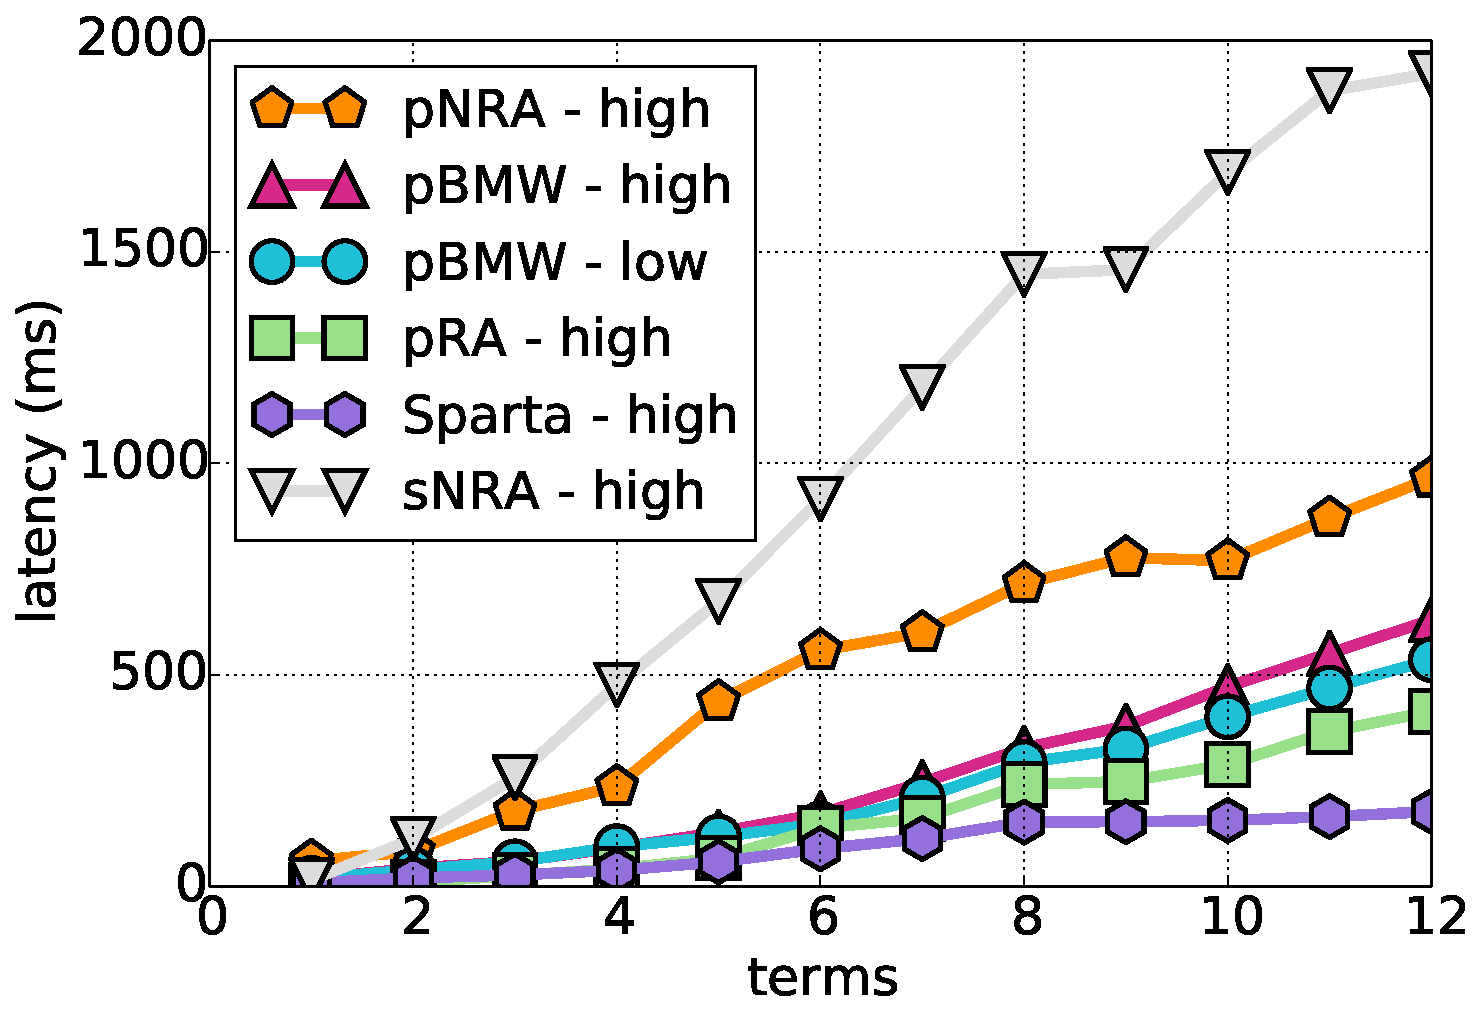
\includegraphics[width=\textwidth]{figures/latency_12threads_clueweb.pdf}
        \caption{Average latency, \cw, high recall algorithms}
        \label{fig:terms-scaling-high-avg}
      \end{subfigure}
     \hfill    
	\begin{subfigure}{0.325\textwidth}
    	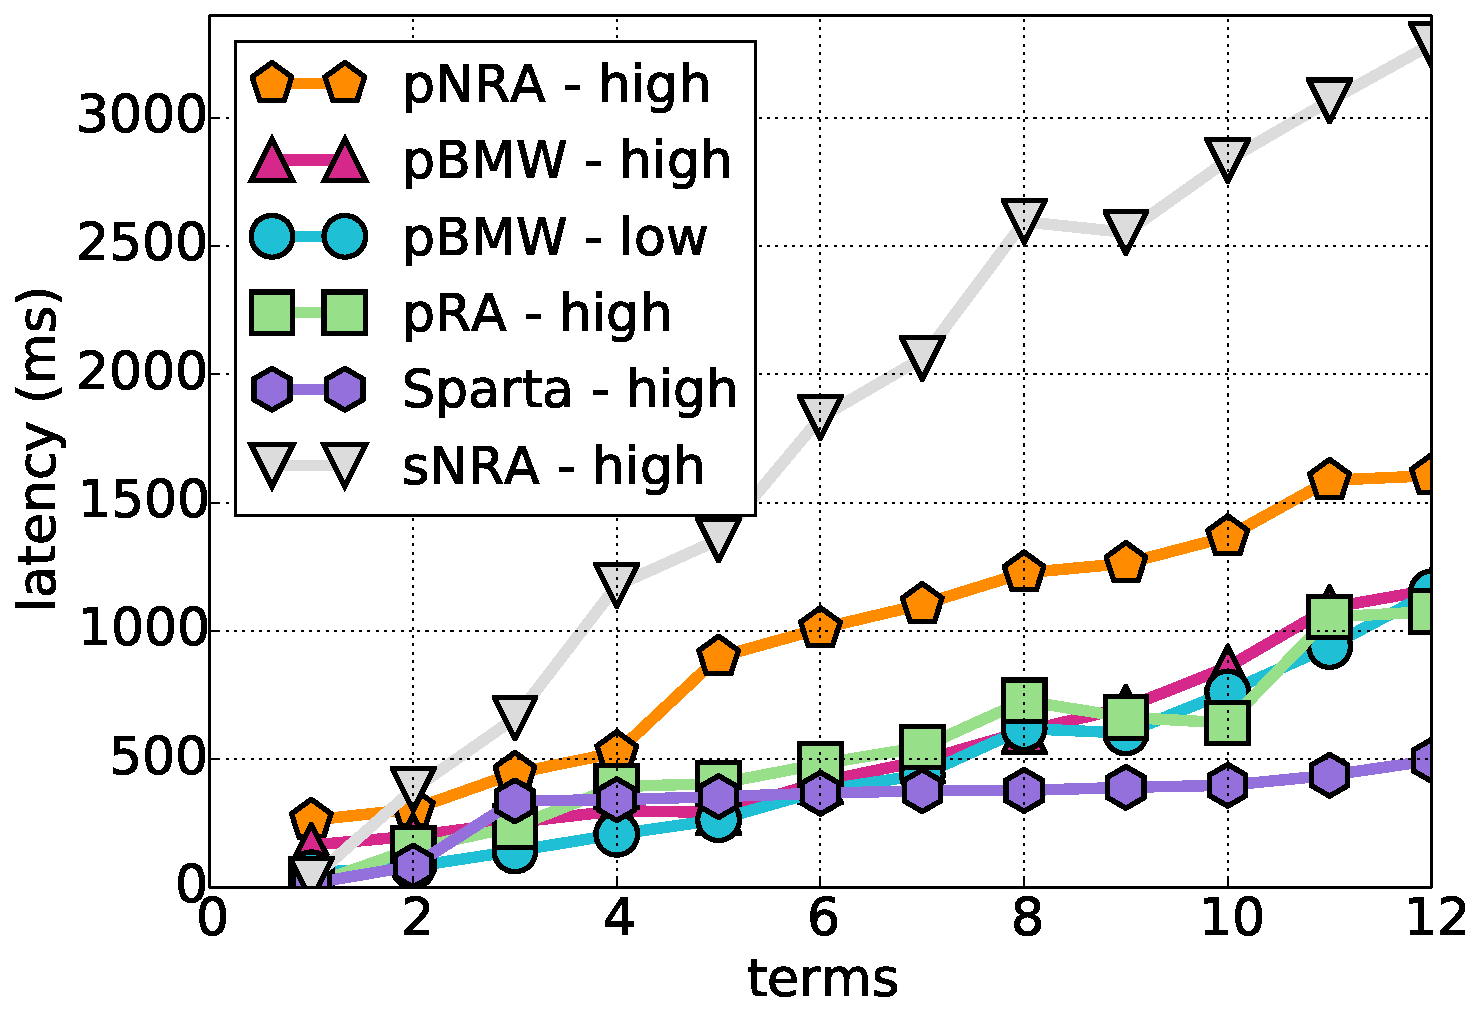
\includegraphics[width=\textwidth]{figures/latency_95th_percentile_clueweb.pdf}
	\caption{95\% latency, \cw, high recall algorithms}
	\label{fig:terms-scaling-high-95}
    \end{subfigure} 
 \hfill
     \begin{subfigure}{0.325\textwidth}
    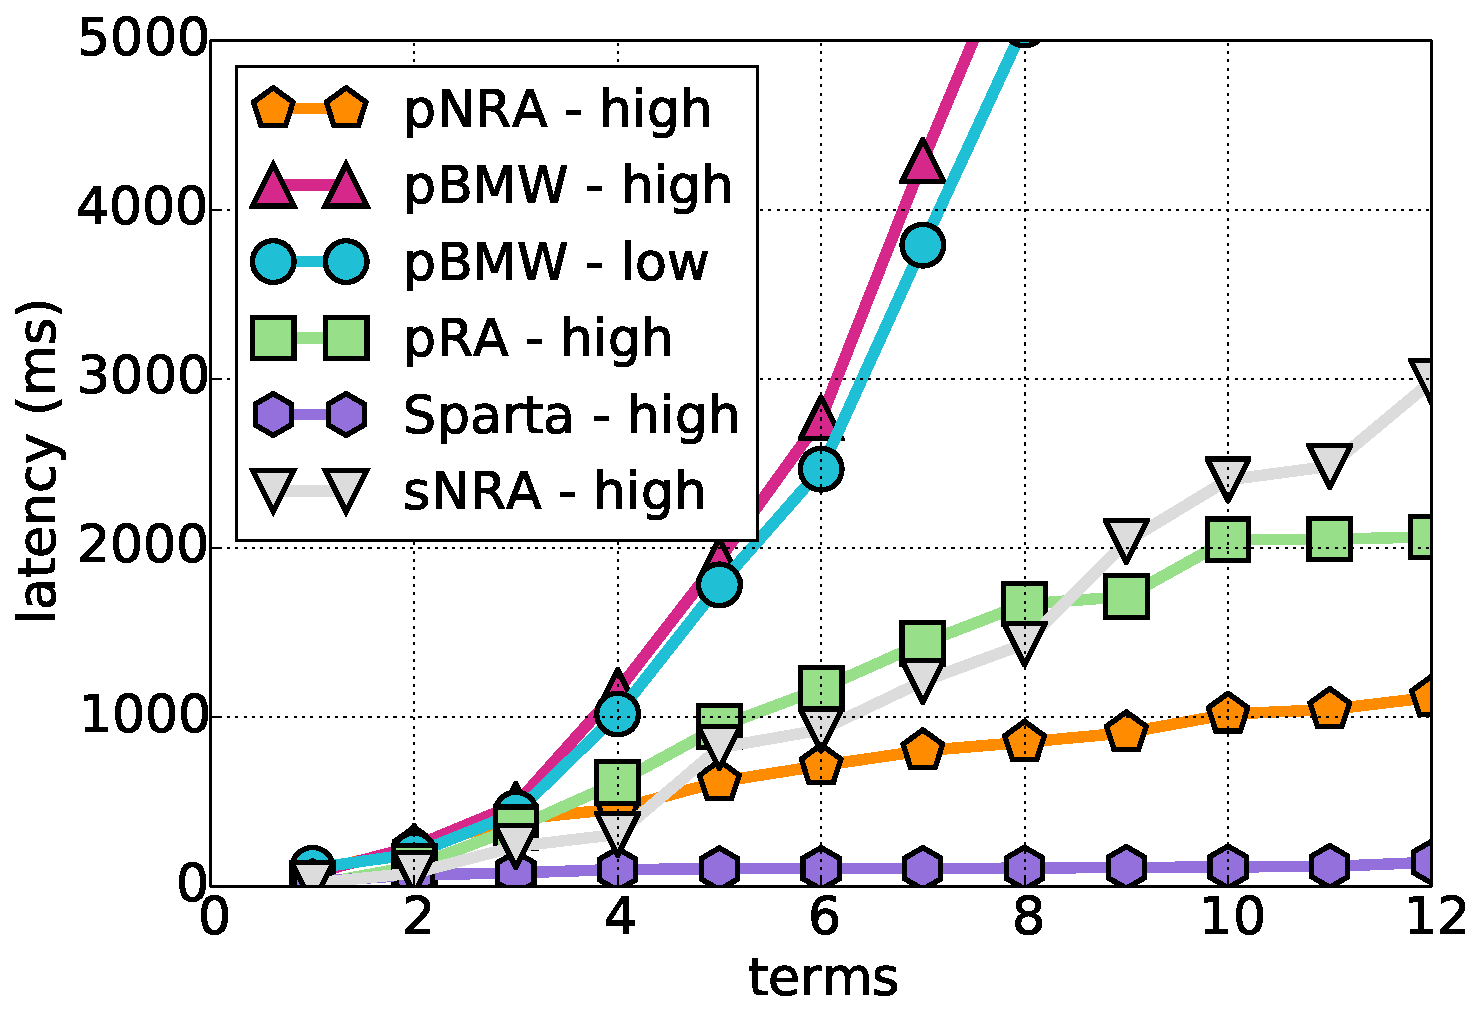
\includegraphics[width=\textwidth]{figures/latency_12threads_cluewebX10.pdf}
	\caption{Average latency, \cwten}
	        \label{fig:terms-scaling-10x-avg}
    \end{subfigure}
    
         

     \begin{subfigure}{0.325\textwidth}
         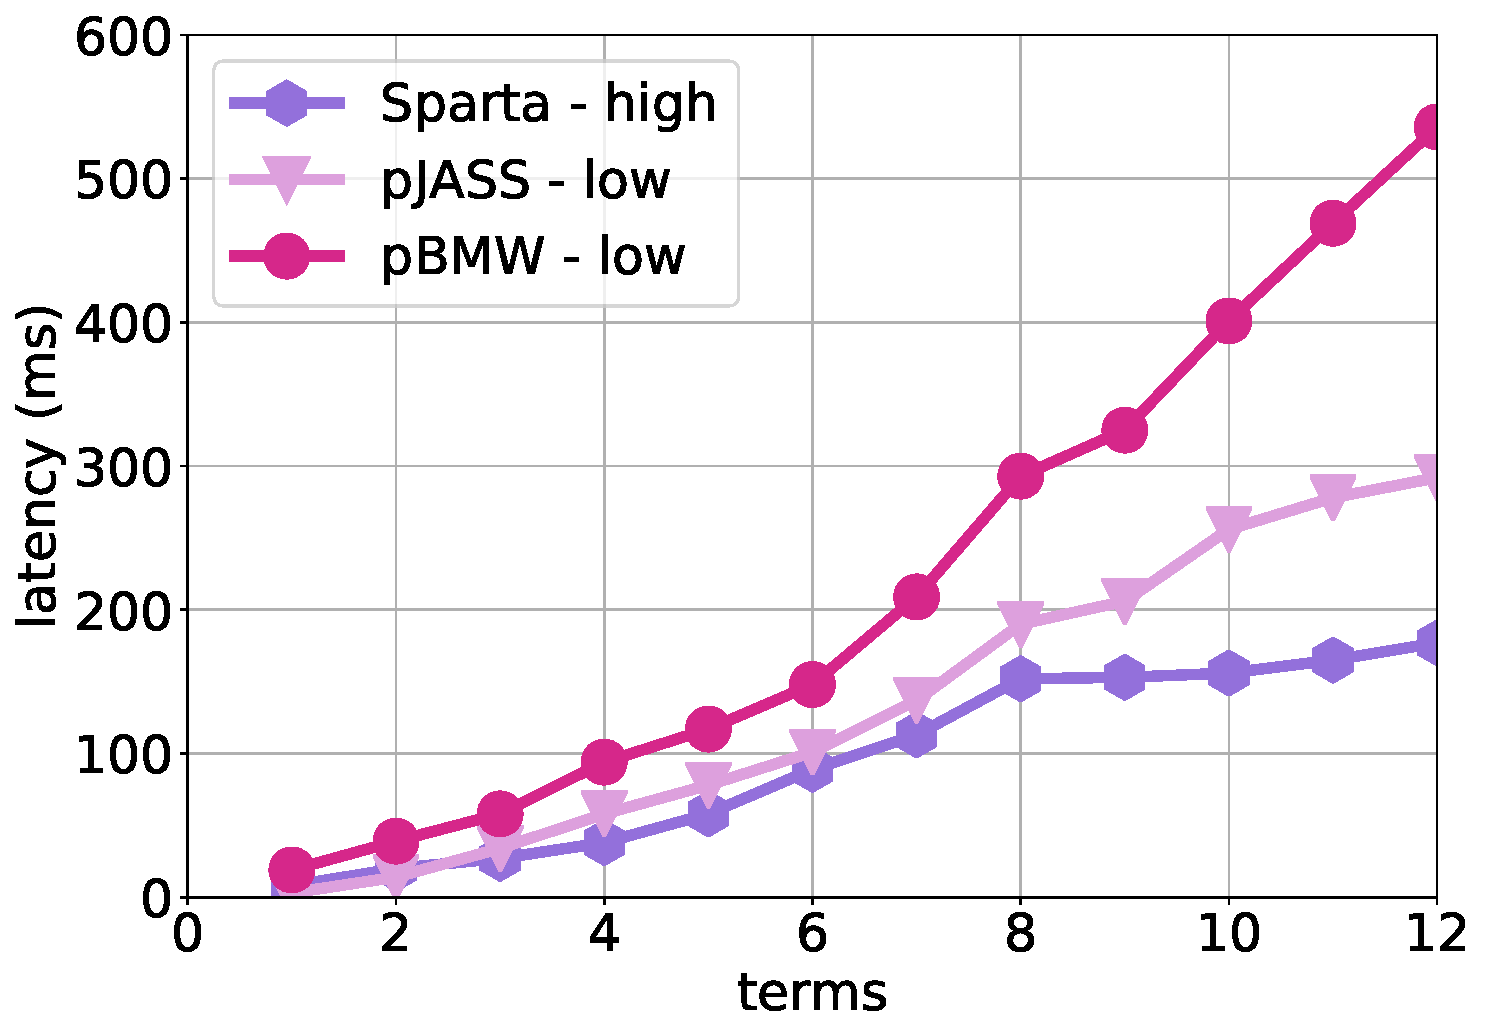
\includegraphics[width=\textwidth]{figures/latency_high_low_12threads_clueweb.pdf}
        \caption{Average latency, \cw, \alg\ vs. low recall algorithms}
        \label{fig:terms-scaling-low-avg}
      \end{subfigure}  
	\hfill
     	\begin{subfigure}{0.325\textwidth}
  	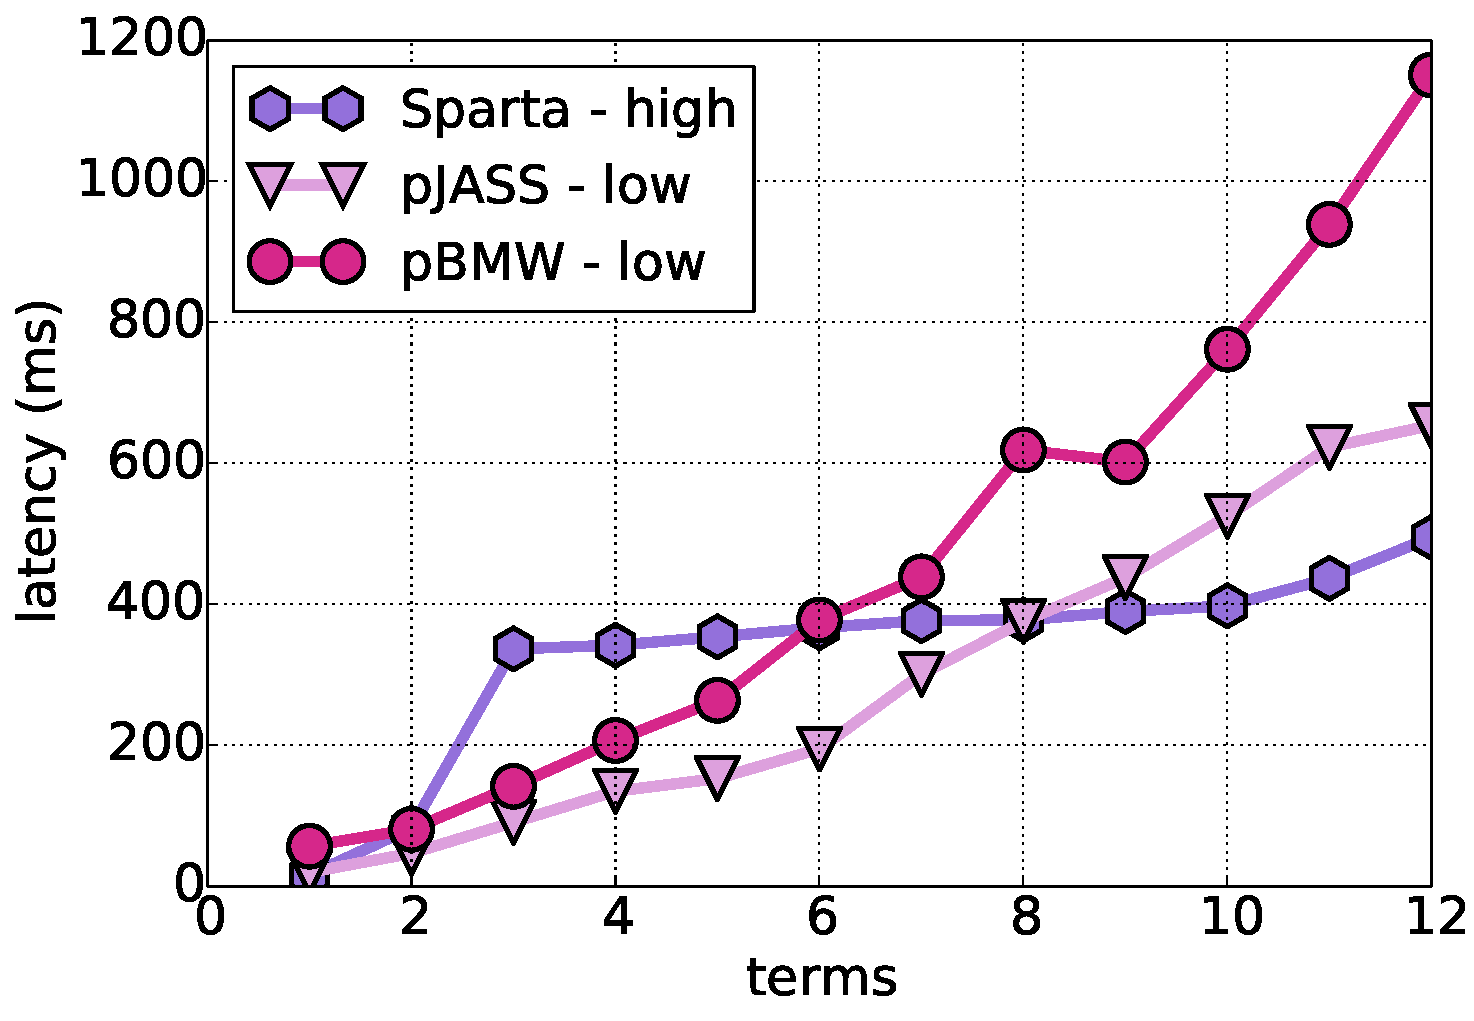
\includegraphics[width=\textwidth]{figures/latency_95th_percentile_high_low_clueweb.pdf}
  	\caption{95\%\bigdataset{, \cw} -- \alg\ vs. low recall algorithms}
	\label{fig:terms-scaling-low-95}
    \end{subfigure}
	\hfill    
      \begin{subfigure}{0.325\textwidth}
         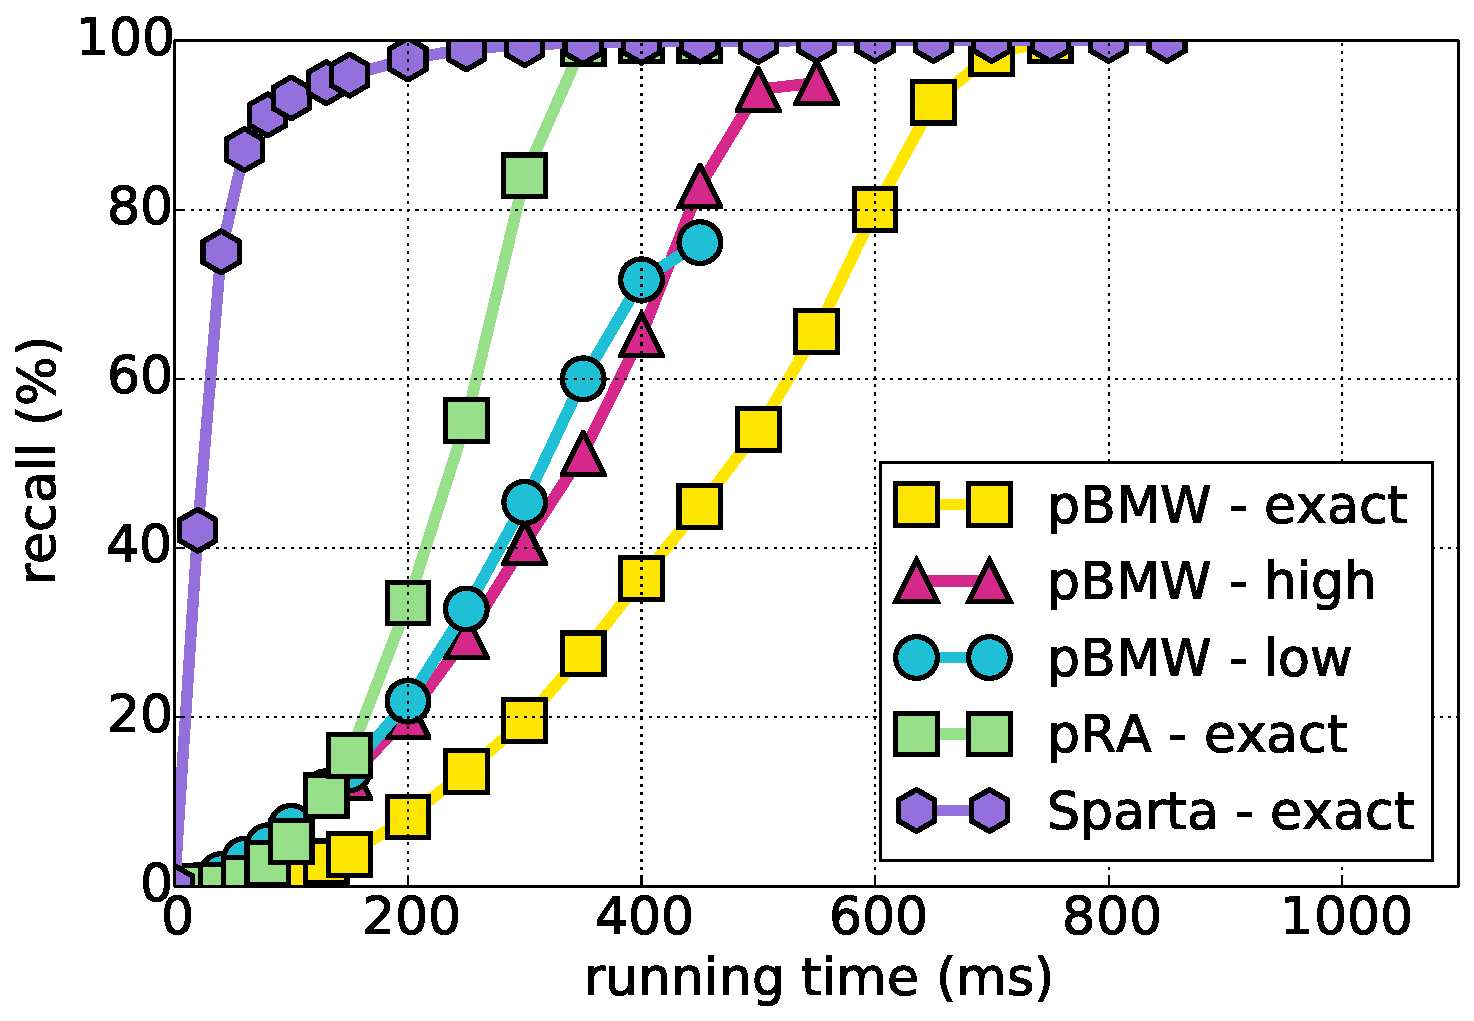
\includegraphics[width=\textwidth]{figures/cumulative_12threads_clueweb.pdf}
        \caption{Recall dynamics, \cw}
        \label{fig:dynamics-clueweb}
      \end{subfigure} 
	
	
      \begin{subfigure}{0.325\textwidth}
      	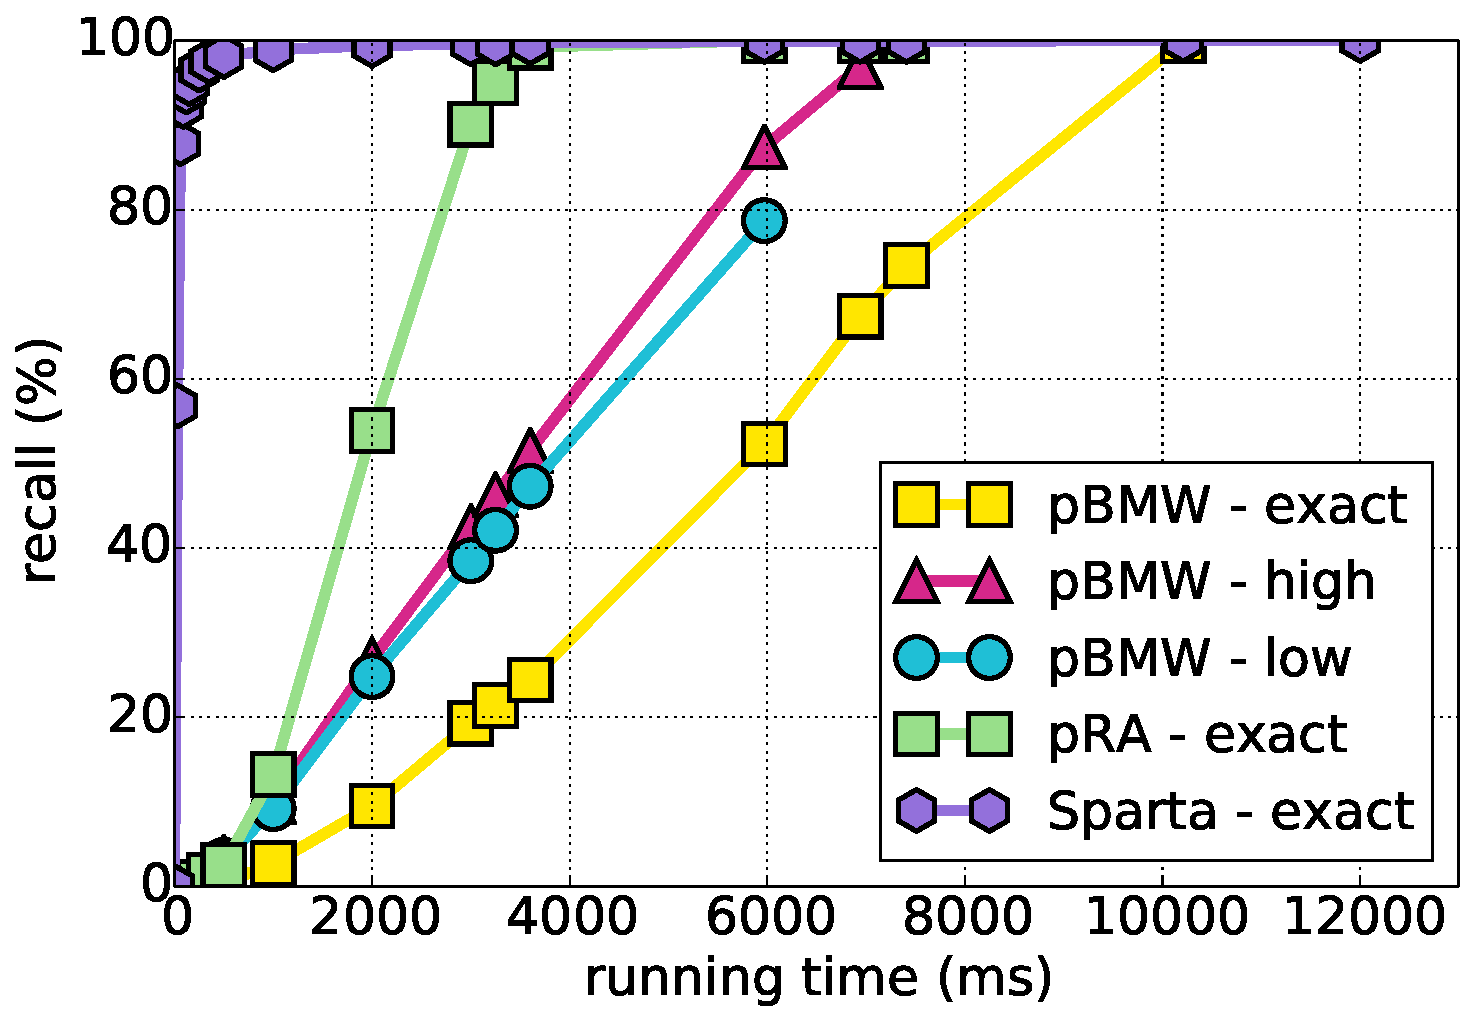
\includegraphics[width=\textwidth]{figures/cumulative_12threads_cluewebX10.pdf}
        \caption{Recall dynamics, \cwten}
	\label{fig:dynamics-cluewebX10}
      \end{subfigure}  
\hfill
      \begin{subfigure}{0.325\textwidth}
         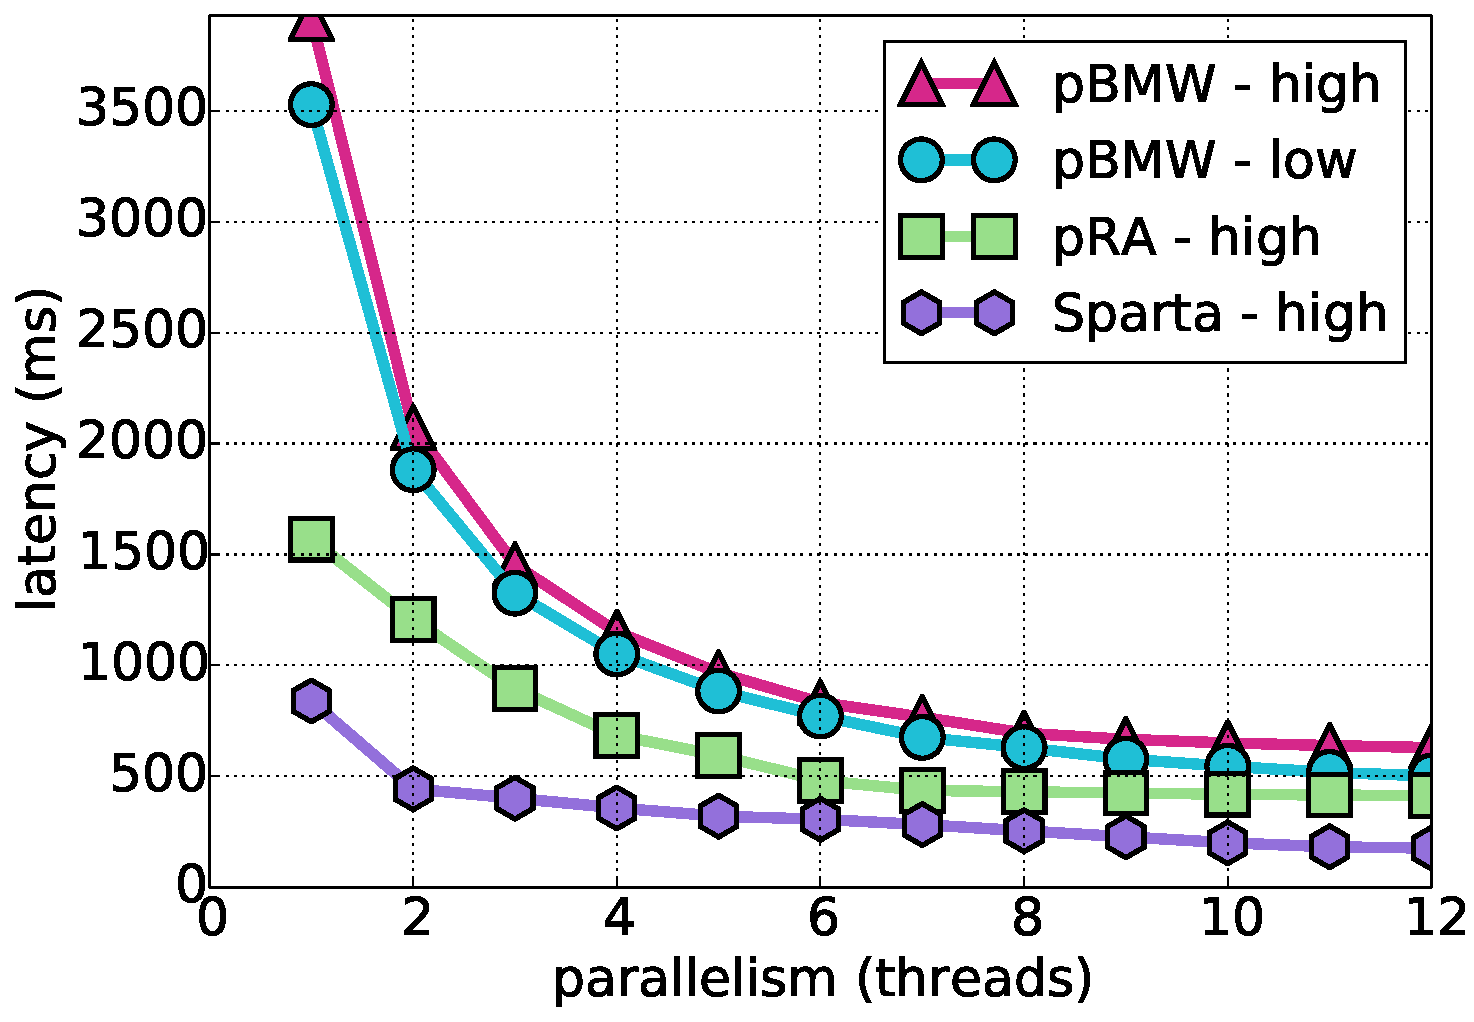
\includegraphics[width=\textwidth]{figures/latency_12terms_clueweb.pdf}
        \caption{Average latency, \cw, 12 terms}
        	\label{fig:threads-scaling-cw}
      \end{subfigure}
\hfill 
      \begin{subfigure}{0.325\textwidth}
      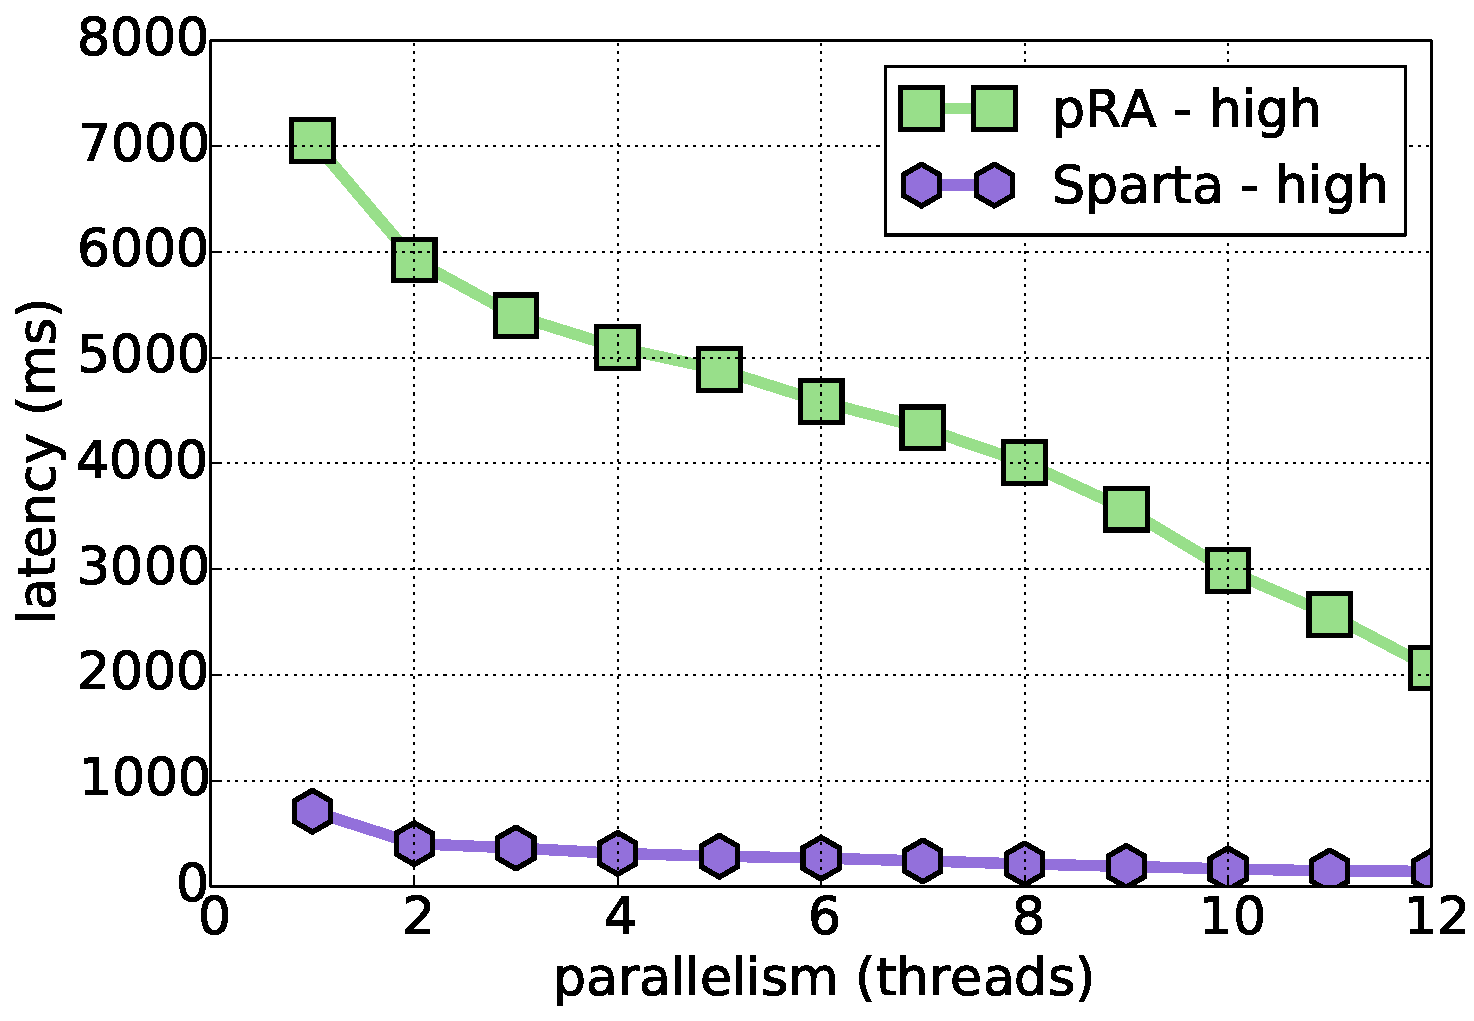
\includegraphics[width=\textwidth]{figures/latency_12terms_cluewebX10.pdf}
	  \caption{Average latency, \cwten, 12 terms}
	  	\label{fig:threads-scaling-cw10}
      \end{subfigure}
      
\caption{Top-k ($k=1000$) query latency. Plots (a)--(e) show scaling with the number of query terms; plots (f)--(g) show recall dynamics with elapsed time for 12-term queries; plots (h)--(i) show scaling with intra-query parallelism.  
%The intra-query parallelism is equal to the number of terms in all plots. 
}
\end{figure*}

%



\remove{
As an aside, note that \pRA\/ scales somewhat better if its whole working set fits into memory. 
However, this is seldom the case when diverse queries are applied to a large index.
%, e.g., when the same small set of queries is evaluated over and over again. 
%This use case is of limited interest.  
%besides, it does not manifest with the \cwten\/ dataset in a statistically significant way. 
} 



On \cw, 
the shared-nothing and unoptimized parallelizations of NRA are weaker than all other alternatives:
\pNRA's  average latency for 12-term queries is $1$ second, and \sNRA's is $1.7$ seconds. 
\bigdataset{
On the larger dataset, \pNRA\ and \sNRA\ are still poorer than \alg\ but perform better than \pBMW. 
This is thanks to the high scalability and early-stopping nature of the approximate NRA approach.
}
These results emphasize the necessity of sharing information among threads (unlike \sNRA) on the one hand,
and the importance of \alg's locality optimizations, (which are missing in \pNRA), on the other. 
Specifically, the background cleaning and local copies of \DMap\ and the lazy updates of \emph{UB} allow \alg\ to benefit from 
local access to data that resides in hardware caches. 
We omit \pNRA\/ and \sNRA\/ from further discussion. 


\paragraph{Recall dynamics.} 
In order to understand how the top-k results get accrued by the different algorithms, we zoom in on the dynamics of query 
recall over the running time. We focus on 12-term queries in a 12-worker configuration. The results are presented in 
Figures~\ref{fig:dynamics-clueweb} and~\ref{fig:dynamics-cluewebX10} for the \cw\/ and \cwten\/ datasets, respectively.
Because the approximate versions of \alg, \pRA, and \pJASS\ are  identical to the respective exact versions until they stop, 
we show the dynamics of the exact versions only.  The same is not true for \pBMW, where $f$ impacts the algorithm's results from the outset.
Hence, we plot all three instances of \pBMW. 
%In the exact algorithms' curves, the rightmost data point corresponds to the exact algorithm's completion time.   

We see that \alg's recall growth is the fastest. For instance, it surpasses $80\%$ recall in less than $50$ ms, 
and $90\%$ recall in less than 100. But over time, its returns  diminish, and most of the work becomes unproductive. Whereas
\pRA\/ takes much longer to converge because it needs to fully score each encountered document,  its concluding phase is faster because 
most relevant documents   have complete  scores. 
\pBMW\/ scans the postings in the order of document ids, which is unrelated to document scores and hence accumulates the true hits 
at a near-linear rate. Obviously, the convergence rate of \pBMW\hi\/ and \pBMW\lo\/ is faster than that of \pBMW\ex. The first 
two accrue results at similar rates until \pBMW\lo\/ stops at approximately $80\%$ recall.
\pJASS's behavior  is similar to \alg's, but it is a bit slower and fails to reach $100\%$ recall within a minute of execution.

%Figure~\ref{fig:terms-scaling}(c) zooms in on \alg's performance versus other variants of NRA: AllPar -- a na\"{\i}ve parallelization  (without the initial sequential phase),  Seq -- a sequential implementation, and SharedState -- a version of \alg\ that does not use local \TMap\/s. Neither of the first two scales with real-time latency. Interestingly, AllPar is slower than Seq, underscoring the importance of aggressive pruning prior to starting the concurrent execution. SharedState is substantially faster, but fails to utilize the hardware cache efficiently due to lack of locality. It thus lags behind \alg\/ by approximately $35\%$ for long queries. 

\paragraph{Parallelism. } 
We next study latency scaling with  intra-query parallelism. 
We  consider  $12$-term queries with a number of threads varying from $1$ to $12$. 
The average latencies appear in Figure~\ref{fig:threads-scaling-cw}
(for \cw) and Figure~\ref{fig:threads-scaling-cw10} (for \cwten). 
\remove{
The latter depicts only \alg\/ and \pRA\/ 
because none of the \pBMW\/ instances scales close to real-time performance.}
The left-most data point in each curve corresponds to the performance of 
the respective sequential algorithm.

\alg\ requires some level of parallelism in order to achieve real-time speed -- its sequential latency is $840$ ms, which is  above typical SLA requirements. Most of the gain is achieved at low-parallelism levels (2 threads suffice). 
The same is true for \pJASS, which hardly improves when afforded more threads, due to unequal thread workloads.
On the other hand, for \pBMW, much higher parallelism is essential -- its latency is inversely proportional to the number of threads. Thus, \alg\ is not only faster 
than \pBMW\ but also requires fewer resources, which benefits throughput as we next show.
%offers the system designer a latency-throughput tradeoff if some slack in latency can be tolerated. 


\paragraph{Throughput. } Finally, we compare the throughput (in queries per second) provided by the different
algorithms. First, we evaluate throughput on fixed query lengths.
Figure~\ref{fig:throughput-scaling} shows the throughput achieved for each query length.
Next, we generate a workload with the query size distribution reported in~\cite{sigir/Guy16},
where the average query length is $4.2$ with a standard deviation of $2.96$. More than $5\%$ of the queries have $10$ or more terms.
The queries are generated as follows: we first sample a query length $\ell$ from the distribution in~\cite{sigir/Guy16}, and then 
select a query uniformly at random among all the length-$\ell$ queries in the complete set of  $1200$ AOL queries. 

Table~\ref{tab:thpt} depicts the results of running this query mix on a shared worker pool  of $12$ threads.
Here too, \alg\/ improves over its competitors, especially on the large dataset, where its throughput is 25x that of \pBMW\hi. 
Its pronounced advantage over \pBMW\ is thanks to a combination of \alg's speed and lower resource utilization.


\begin{figure}[tbh]
\centering
\begin{tabular}{ccc}
      \begin{subfigure}[t]{0.32\textwidth}
         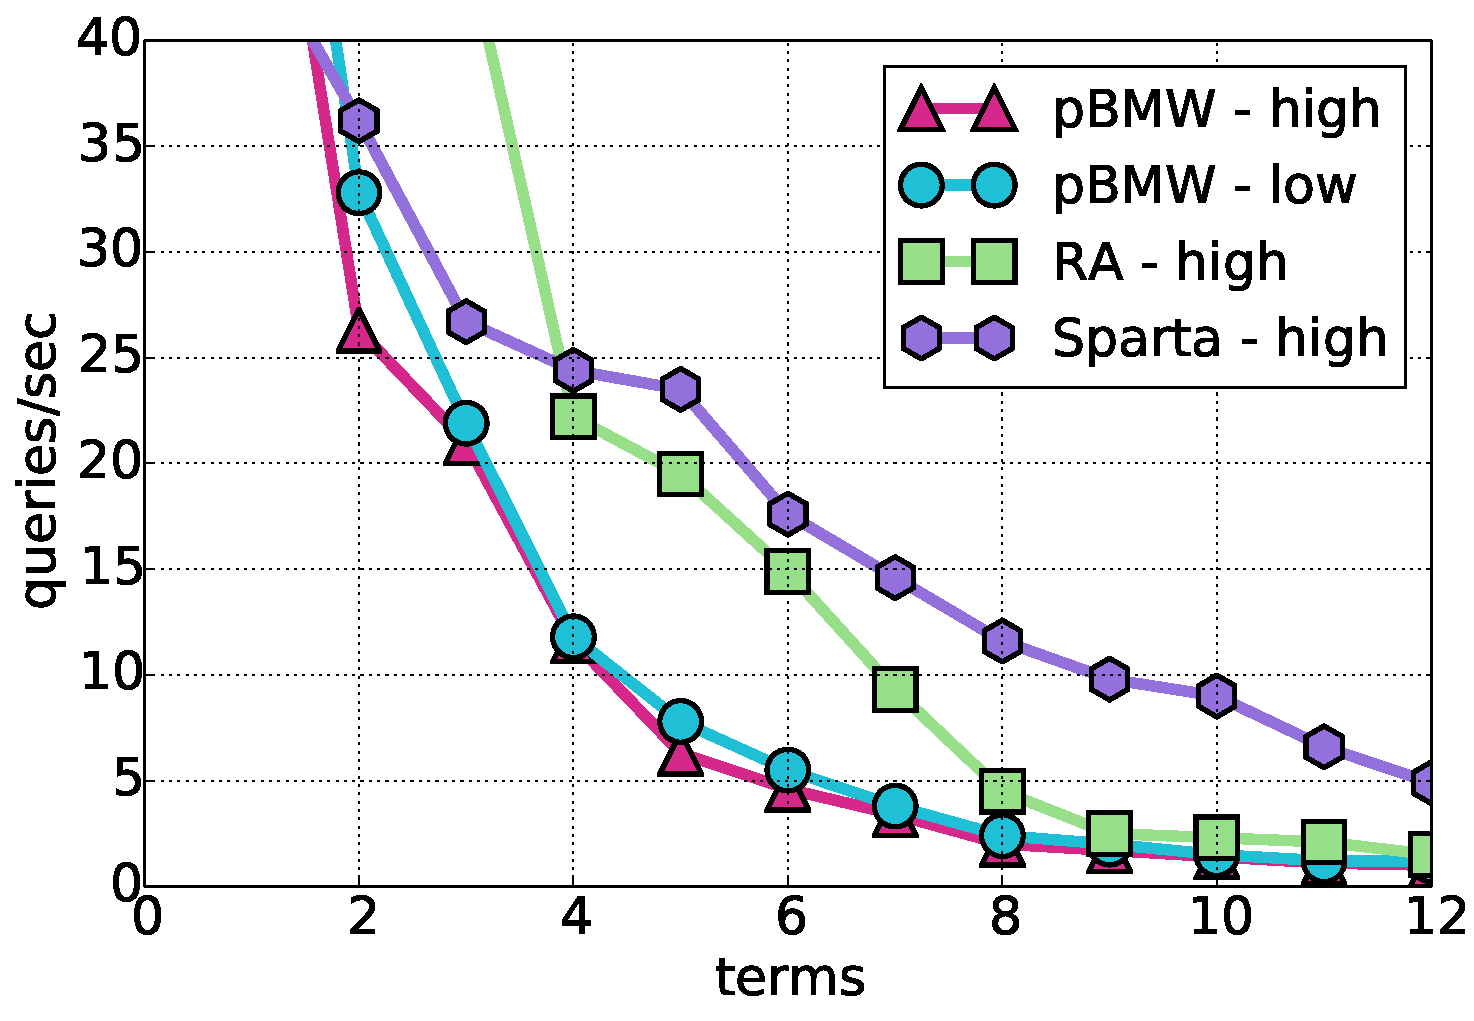
\includegraphics[width=\textwidth]{figures/throughput_12threads_clueweb.pdf}
      \end{subfigure}      
\end{tabular}
\caption{Top-k query throughput scaling with the number of query terms, \cw. The intra-query parallelism 
is equal to the number of terms in all parallel algorithms.}
\label{fig:throughput-scaling}
\end{figure}



\begin{table}[htb]
\centering
\begin{tabular}{ l | c  c   c  c }
%\hline
               & \alg  &  \pRA  & \pBMW  & \pJASS \\  \hline
   \cw      &  12.5 &  10.9 & 5.95 & 10.8 \\ %\hline
   \cwten & 9.6  & 1.8    & 0.38  & N/A \\ %\hline
\end{tabular}
\caption{Average throughput (in queries per second) of the approximate high recall algorithms on a query distribution measured for voice queries in production. }
\label{tab:thpt}
\end{table}
 
\section{Related Work}
\label{sec:related}

Verbose queries challenge standard top-k processing techniques in terms of runtime latency. Huston and Croft \cite{Huston:2010} evaluated several sequential query processing techniques for verbose queries, concluding that the most effective one is to simply reduce the length of the query by omitting stop-words or ``stop-structure'' expressions. 
In this work we ignore the query pre-processing phase and consider the query as a bag of words given after textual analysis.

Crane et al.~\cite{Crane:2017} showed that document-at-a-time processing algorithms are susceptible to tail queries that may take orders of magnitude longer than the median query. Additionally, approximate query evaluation in WAND and BMW does not significantly reduce the variance. Moreover, in agreement with our findings, they showed that score-at-a-time algorithms, which access the  posting lists in decreasing impact order, are less sensitive to tail queries due to their effective early termination capability. 

With the rapid development in multiprocessor hardware, a new line of research has emerged on exploiting multi-threaded programing for top-k retrieval. Tatikonda 
et al.~\cite{Tatikonda:2011} studied parallel top-k retrieval for web queries that are processed in conjunctive mode. They improved the performance of posting list intersection by considering various coarse-grained and fine-grained parallelization models. The work associated with a given query was partitioned into a number of small and independent tasks that were subsequently processed in parallel.  Similarly, Bonacic et al.~\cite{Bonacic:2010} parallelized the query processing by dividing the document space into chunks; each chunk of the inverted file was assigned to a thread, which identified the (local) top-k results of that portion using WAND. Finally, a broker aggregated the top results of all threads for extracting the final output. 

Rojas et al.~\cite{rojas2013efficient} proposed a multi-threaded implementation for BMW. Similarly to \cite{Bonacic:2010}, each thread applies BMW over a portion of the inverted file in order to identify the (local) top-k results. In one implementation, each thread maintains a local heap. Alternatively, a global heap is shared by all threads, and so no final merge is needed. More importantly, the global threshold, which is the current minimum document score in the heap, is available to all threads. The global threshold is much tighter than the threads' local thresholds, hence much less work is done by each of the threads as  more documents can be safely skipped. However, additional locks are needed to guarantee exclusive updates of the shared heap. The experimental results described in \cite{rojas2013efficient} show the superiority of the local-heap over the global-heap version. The pBMW implementation used in our experiments follows the local-heap version described above,
but periodically shares the  $\Theta$ values among the threads for improved performance.

Jeon et al.~\cite{Jeon:2014} argued that parallelizing the processing of an individual query gives limited benefits compared to sequential execution since short-running queries, which dominate the workload, do not benefit from parallelization. On the other hand, parallelization substantially reduces the execution time of long-running queries.  They presented an adaptive resource management algorithm that chooses the degree of parallelism at runtime for each query, based on predicting high-latency queries.

%DC not related:
Ao et al.~\cite{Ao:2011} explored using GPU hardware for information retrieval. They focused on optimizing throughput rather than latency. 

The Threshold Algorithm and its variants \cite{Fagin:2001,Fagin:2003,Akbarinia:2007} have been extensively studied by the database community, and have been applied in many relational database systems (for a comprehensive survey see \cite{ilyas2008survey}). 
Mamoulis et al.~\cite{Mamoulis:2007} observed two main phases during NRA processing -- the ``growing phase'', where the candidate list grows, and the ``shrinking phase'' where no new documents can end up in the top-k results, after the first stopping condition is met. They used different data structures for the two phases in order to minimize the number of accesses and the memory requirements. 
Gursky et al.~\cite{Gursky:2008} also noticed the bottleneck in NRA computation derived from NRA's needs to maintain an extremely large number of partially scored candidates. They proposed several optimization methods for candidate list maintenance to speed up the search. One of their suggested approaches is to periodically remove irrelevant candidates from the candidate list, in a similar manner to \alg{}. 
%In contrast, \alg{} handles this bottleneck by dedicating a specific cleaning thread that keeps removing irrelevant candidates during the search process. 

Yuan et al.~\cite{yuan:2012} observed that the number of accesses to the sorted lists by NRA could be further reduced by selectively performing the sorted accesses to the different lists (instead of in parallel). They proposed a selection policy that prioritizes the accesses to the sorted lists and cuts down unnecessary accesses. They showed significant cutoff in the number of accesses with respect to the original NRA. However, 
%this algorithm is not safe. Moreover, 
as the authors pointed out, the effectiveness of this approach in terms of run-time latency still has to be explored.

In the IR setting, TA has received much less attention. A few exceptional examples are
\cite{Theobald:2004,Bast:2006,Theobald:2008}, which experimented with TA on web data  using standard IR metrics. Bast et al.~\cite{Bast:2006} optimized the TA scheduling method based on a cost model for sequential and random accesses. Theobald et al.~\cite{Theobald:2008} extended TA for XML query languages. Another work by Theobald et al.~\cite{Theobald:2004} introduced an approximate TA algorithm based on probabilistic arguments: When scanning the posting lists in descending order of local scores, various forms of derived bounds are employed to predict when it is safe, with high probability, to skip candidate items hence trading off accuracy for sorted access. Applying similar probabilistic pruning rules for Sparta  may prove beneficial and is left for future work.


%Gong et al. \cite{Gong:2010} proposed a distributed version of the TA algorithm. It partitions the original inverted files into sub-files . Each process retrieves the top-k results in its portion independently using TA algorithm, and the results from all portions are then merged to provide the final top-k answers. 
 

 
% %%%%%%%%%%%%%%%%%%%%%%%%%%%%%%%%%%% 
\section{Conclusions}
\label{sec:conclusions}

We presented \alg, a practical algorithm for approximate top-k retrieval on server-grade multi-core hardware. 
To our knowledge, \alg\ is the first algorithm capable of serving  long queries ($10$ or more terms)
within interactive latency bounds.
\alg\ can therefore support modern search experiences -- which induce long queries -- within real-time SLA requirements. 


\alg\ leverages the efficiency and early-stopping properties of the seminal Threshold Algorithm. 
It forgoes the need for random access and duplicate indices by using the  TA's 
NRA variant. 
It achieves high performance by 
optimizing memory footprints, memory access patterns, inter-thread data sharing, and synchronization.  

\alg\/ yields sub-$180$ ms average latencies on standard hardware for queries of up to $12$ terms when applied 
to large data sets of $50$M and $500$M documents. 
  It does so while producing a highly accurate approximation of the exact results 
(a recall of above $97.5\%$). 
\inred{
For comparison, its state-of-the-art parallel competitors, \pBMW\/ and \pJASS,  
required $640$ ms and above 1 second, respectively, to provide similar accuracy.
 }



\clearpage
%\bibliographystyle{ACM-Reference-Format}
\bibliography{references}  


\end{document}
